\documentclass{article}
\usepackage{graphicx}
\graphicspath{ {./images/} }
\usepackage[export]{adjustbox}

\title{IS Praktiskais darbs 2023}
\author{Gunārs Ābeltiņš}
\date{2022-06-05}

\begin{document}

\maketitle

\section{Datu kopas nosaukums}
Consumers - monthly data [ei\_bsco\_m].General economic situation over the last 12 months

\section{Problēmas formulējums analīzei}
Kāda ir patērētāju uzskats par ekonomisko situāciju pēdējo 12 mēnešu laikā, salīdzinot baltijas valstis ar eiropu.

\section{Analītiskās atskaites izveides apraksts}
\subsection{Datu sagatavošana}
Ieguvu datus no "EU open data portal” ka .xlsx failu.

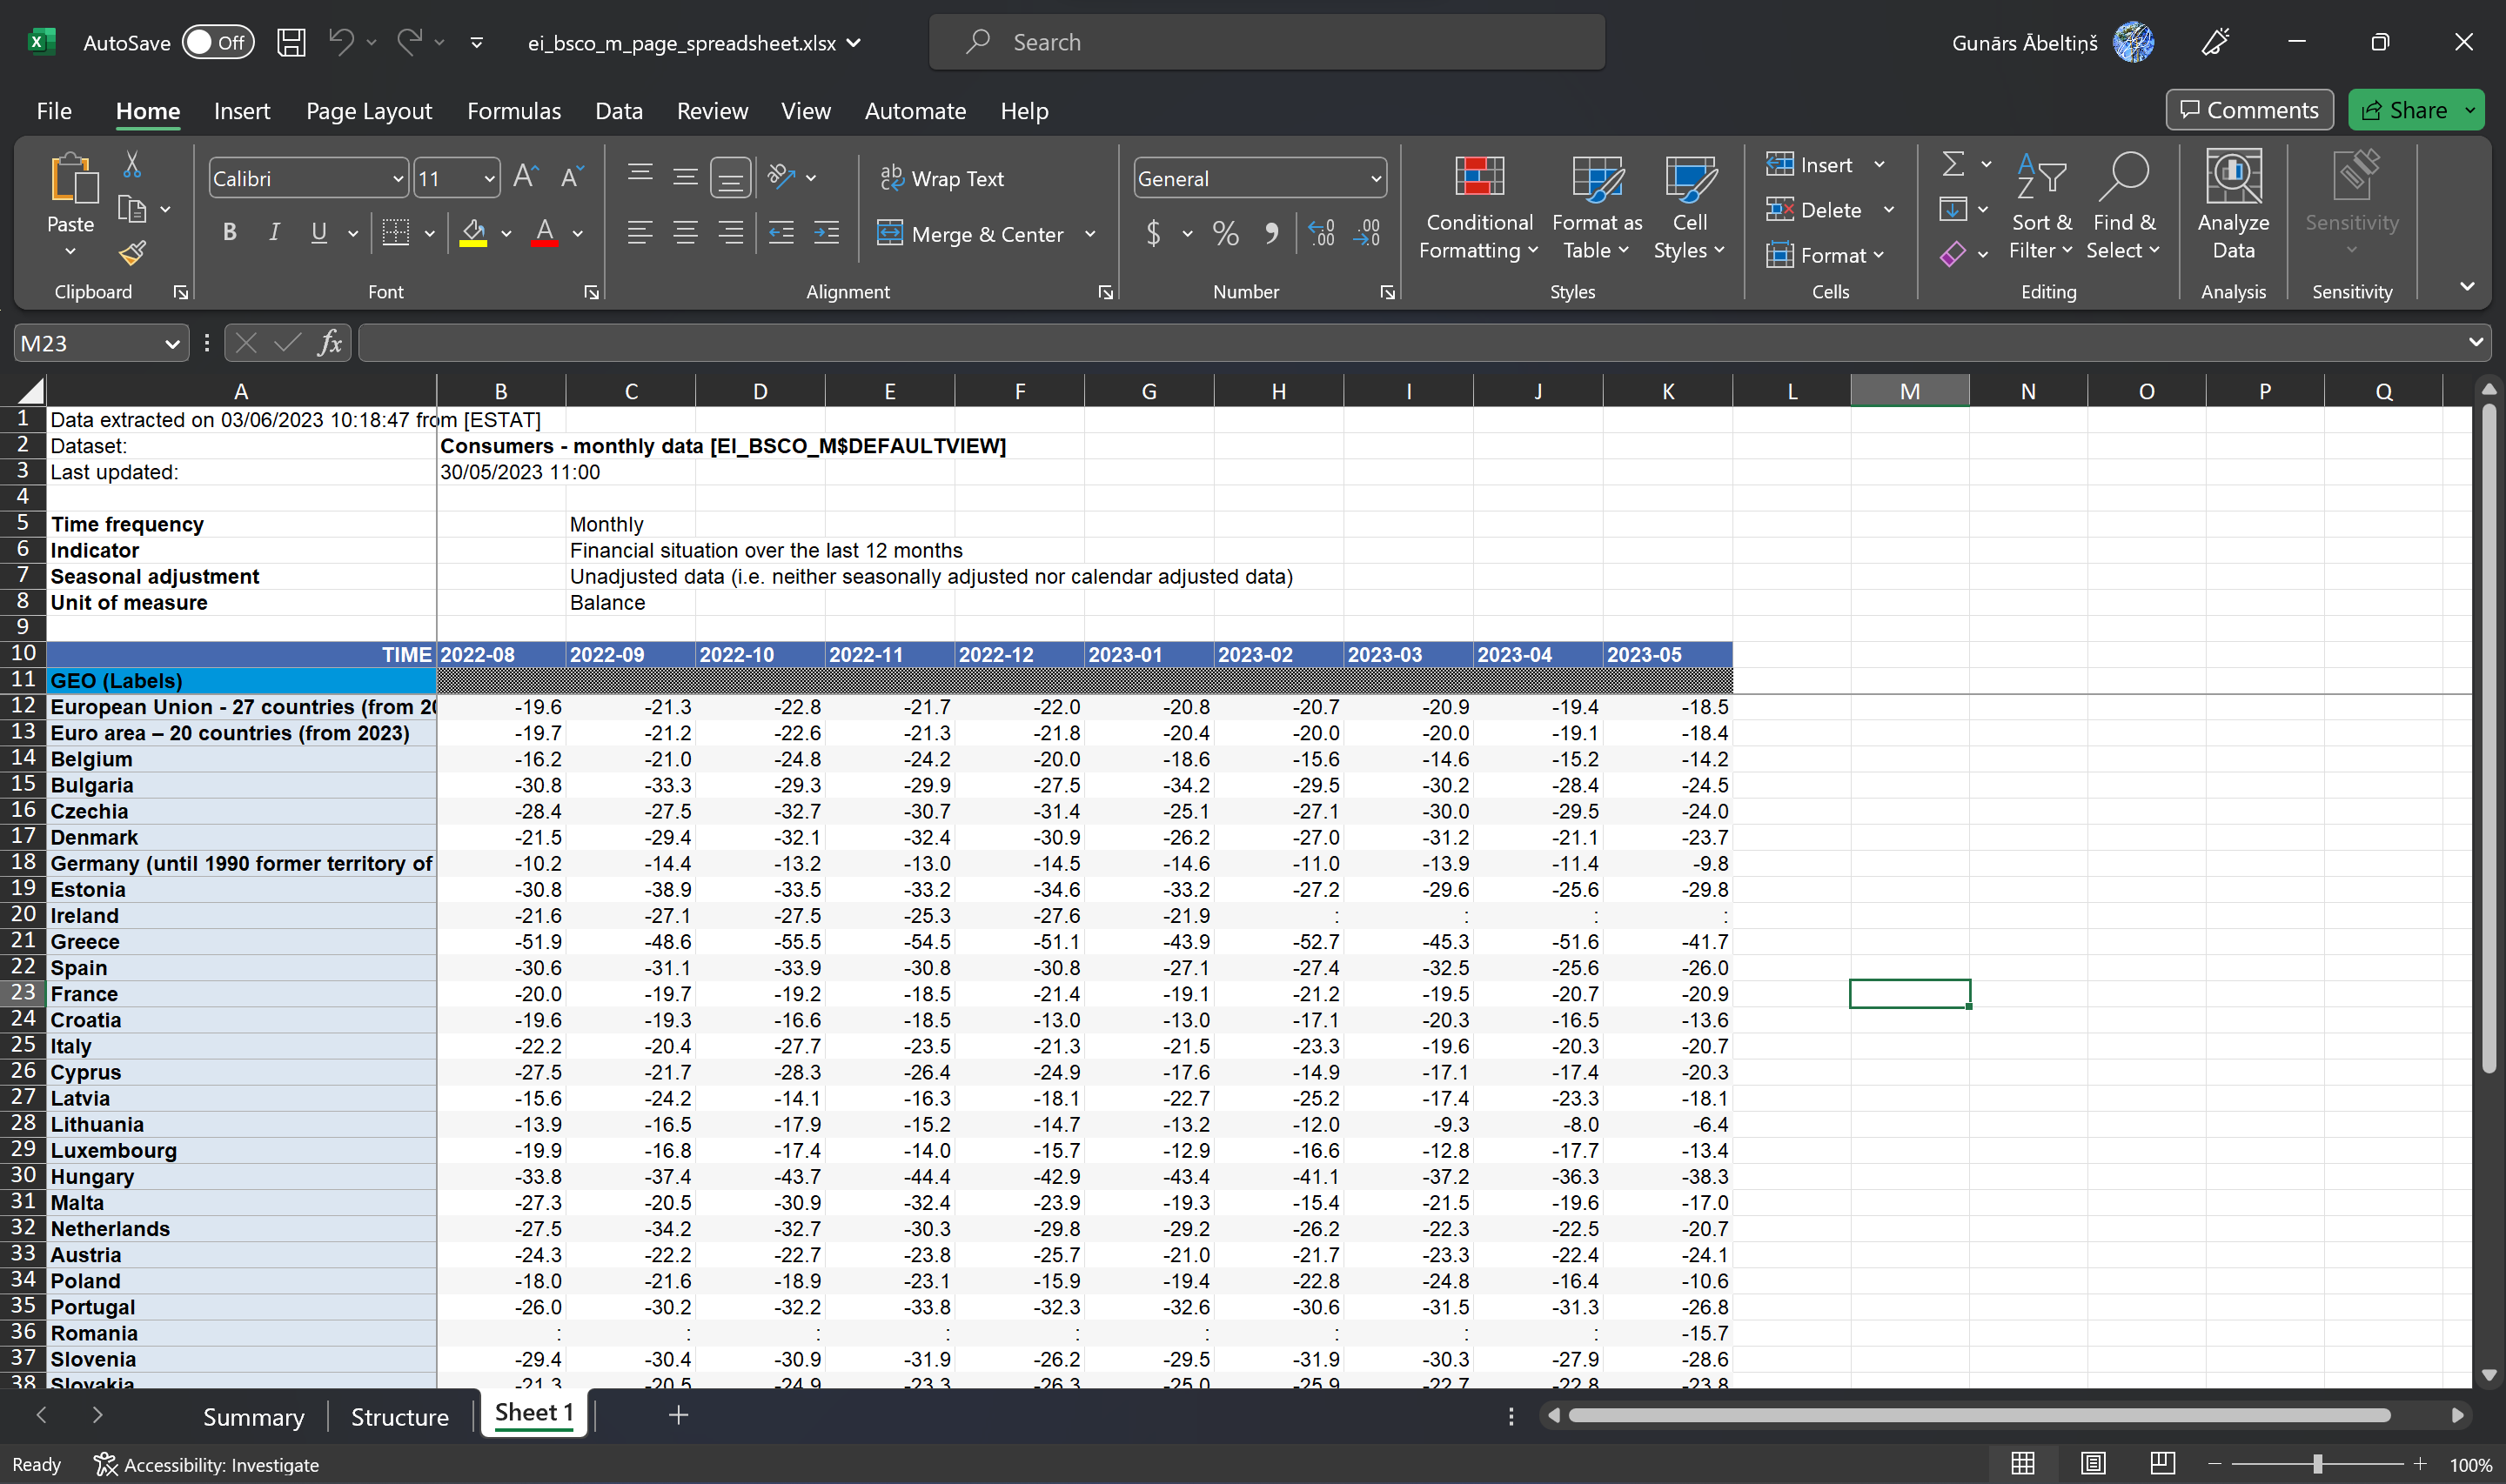
\includegraphics[width=0.9\textwidth, center]{Excel}

Pārveidoju datus, lai būtu iespējams no tiem ģenerēt atskaites.

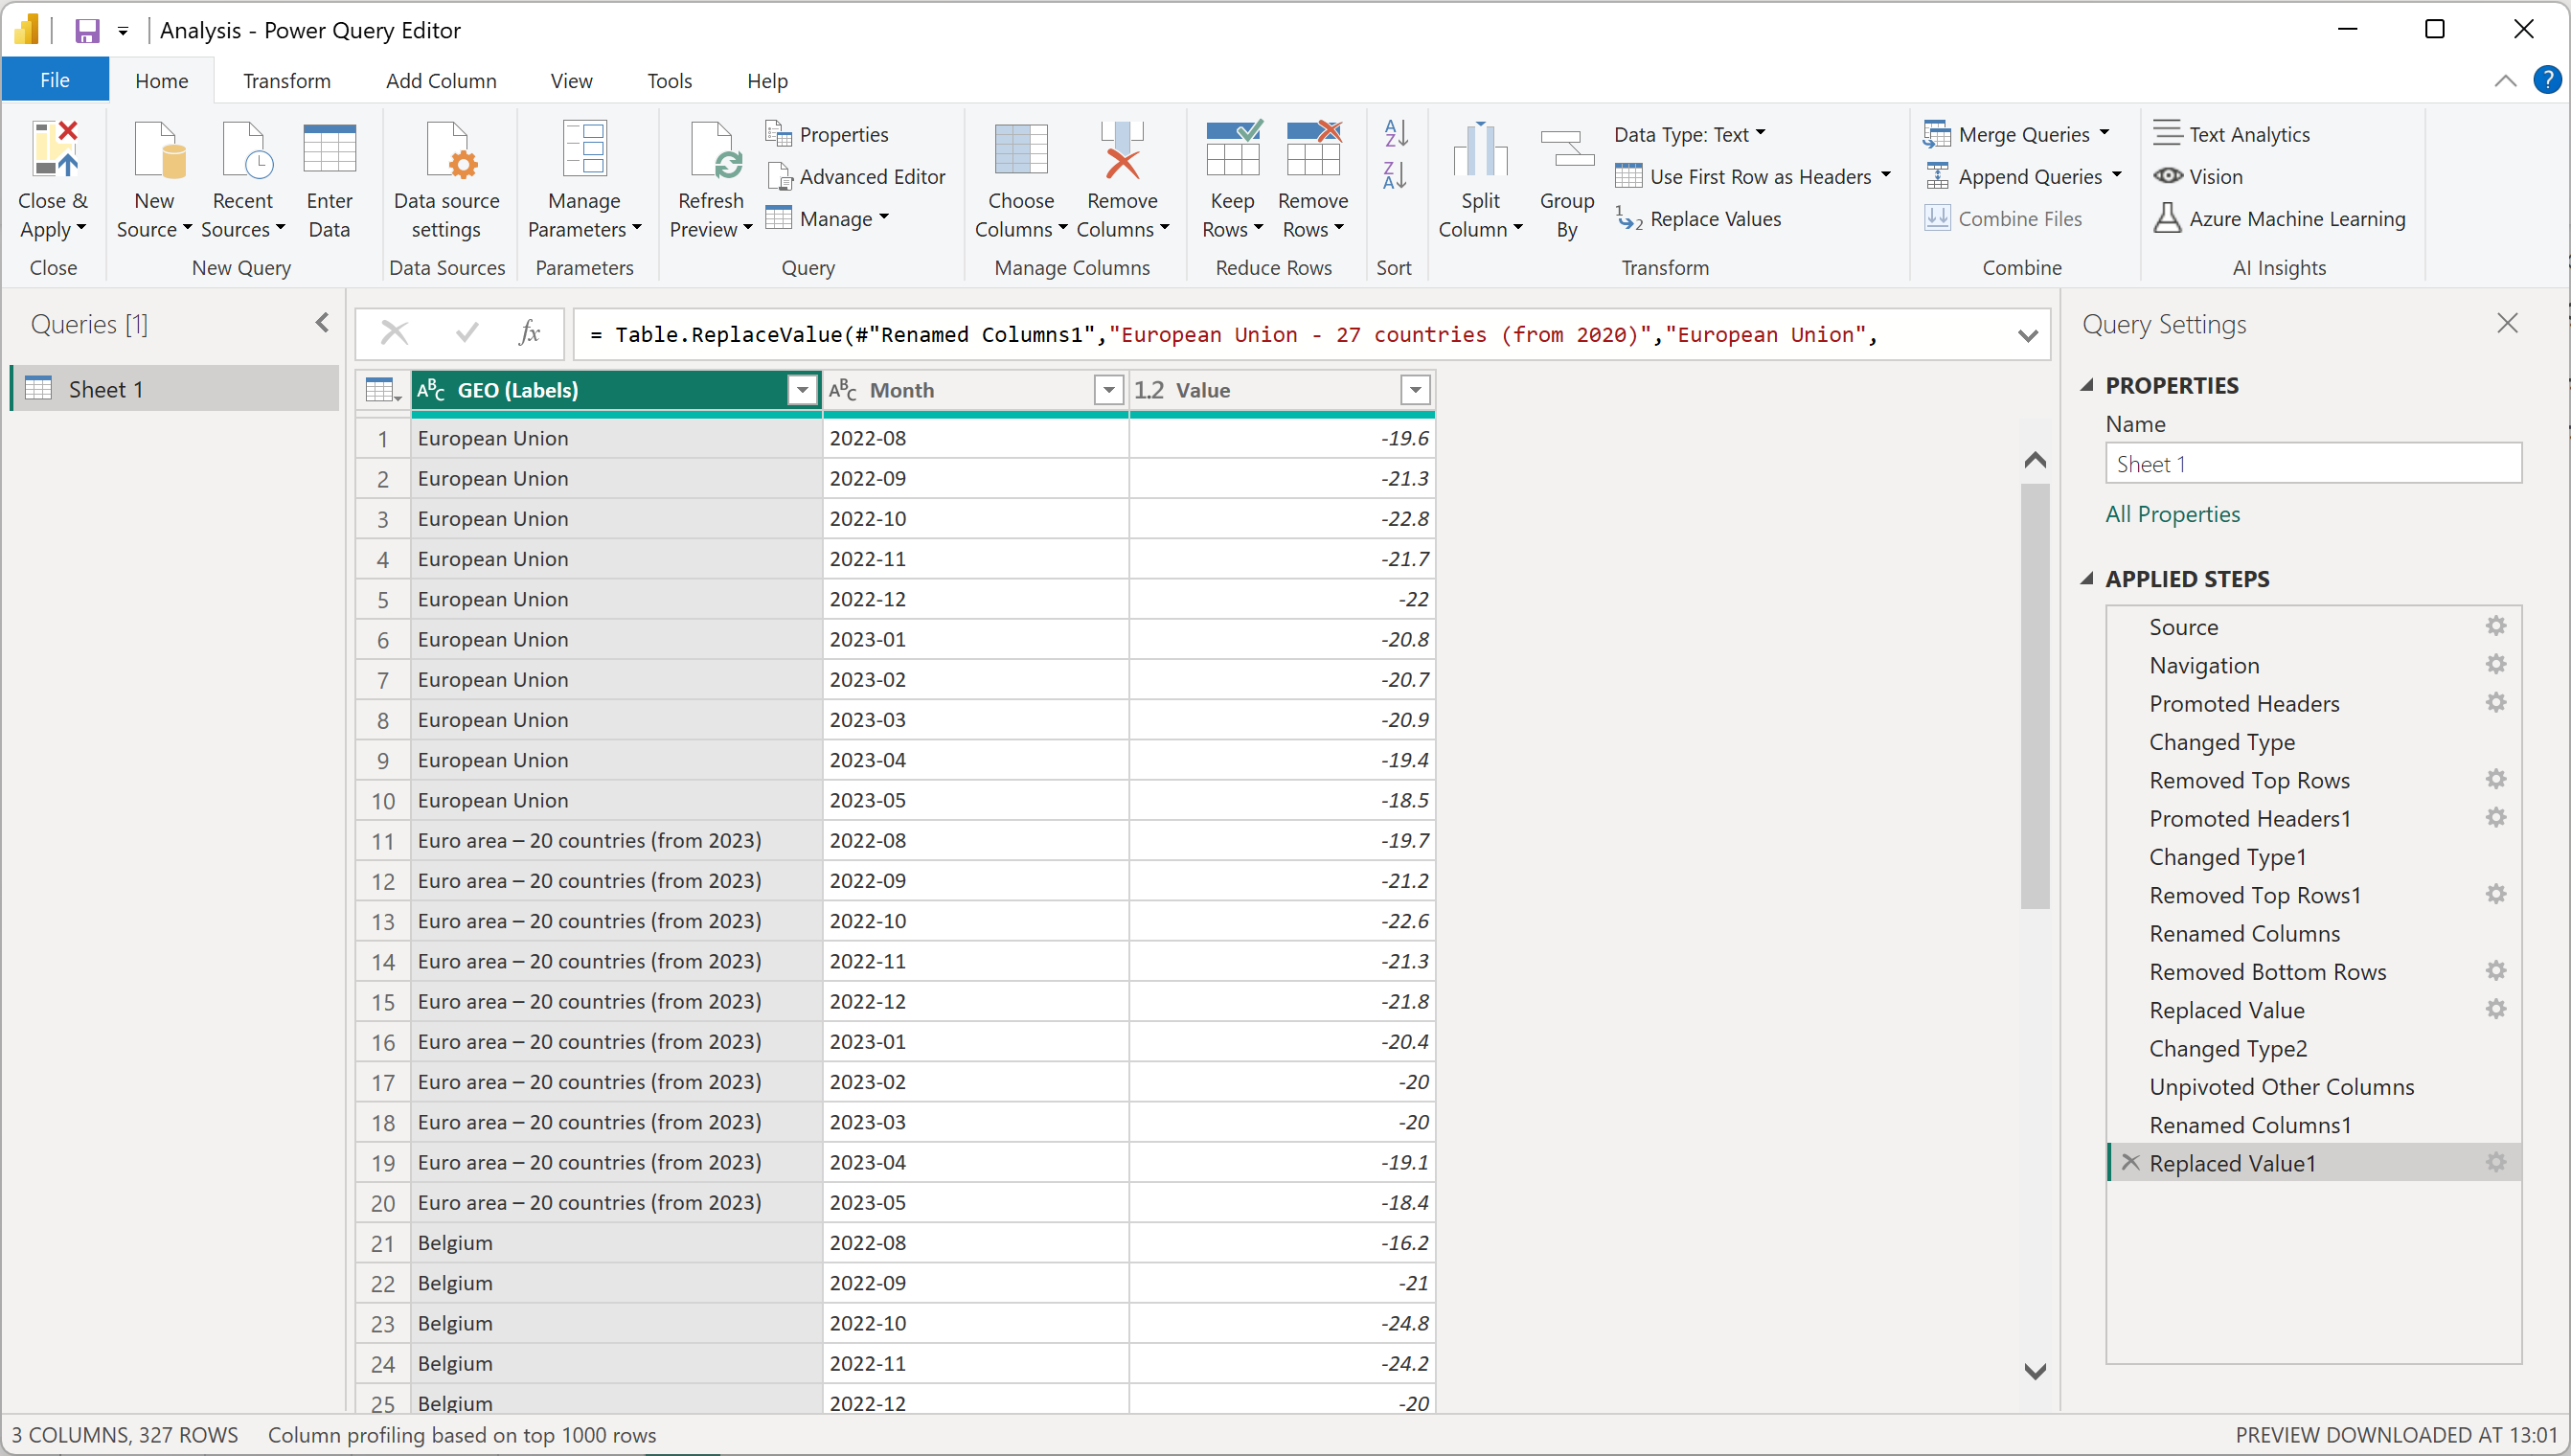
\includegraphics[width=0.9\textwidth, center]{Transform}

\subsection{Atskaišu ģenerēšana}
\subsubsection{Kartes diagramma}
Pirmā diagrama, ko veidoju ir kartes diagrama, lai redzētu kāda ir situācija baltijas valstīs un eiropā. Un varētu ievērot iespējamas sakarības, kas atkarigs no valsts ģeogrāfiska novietojuma.

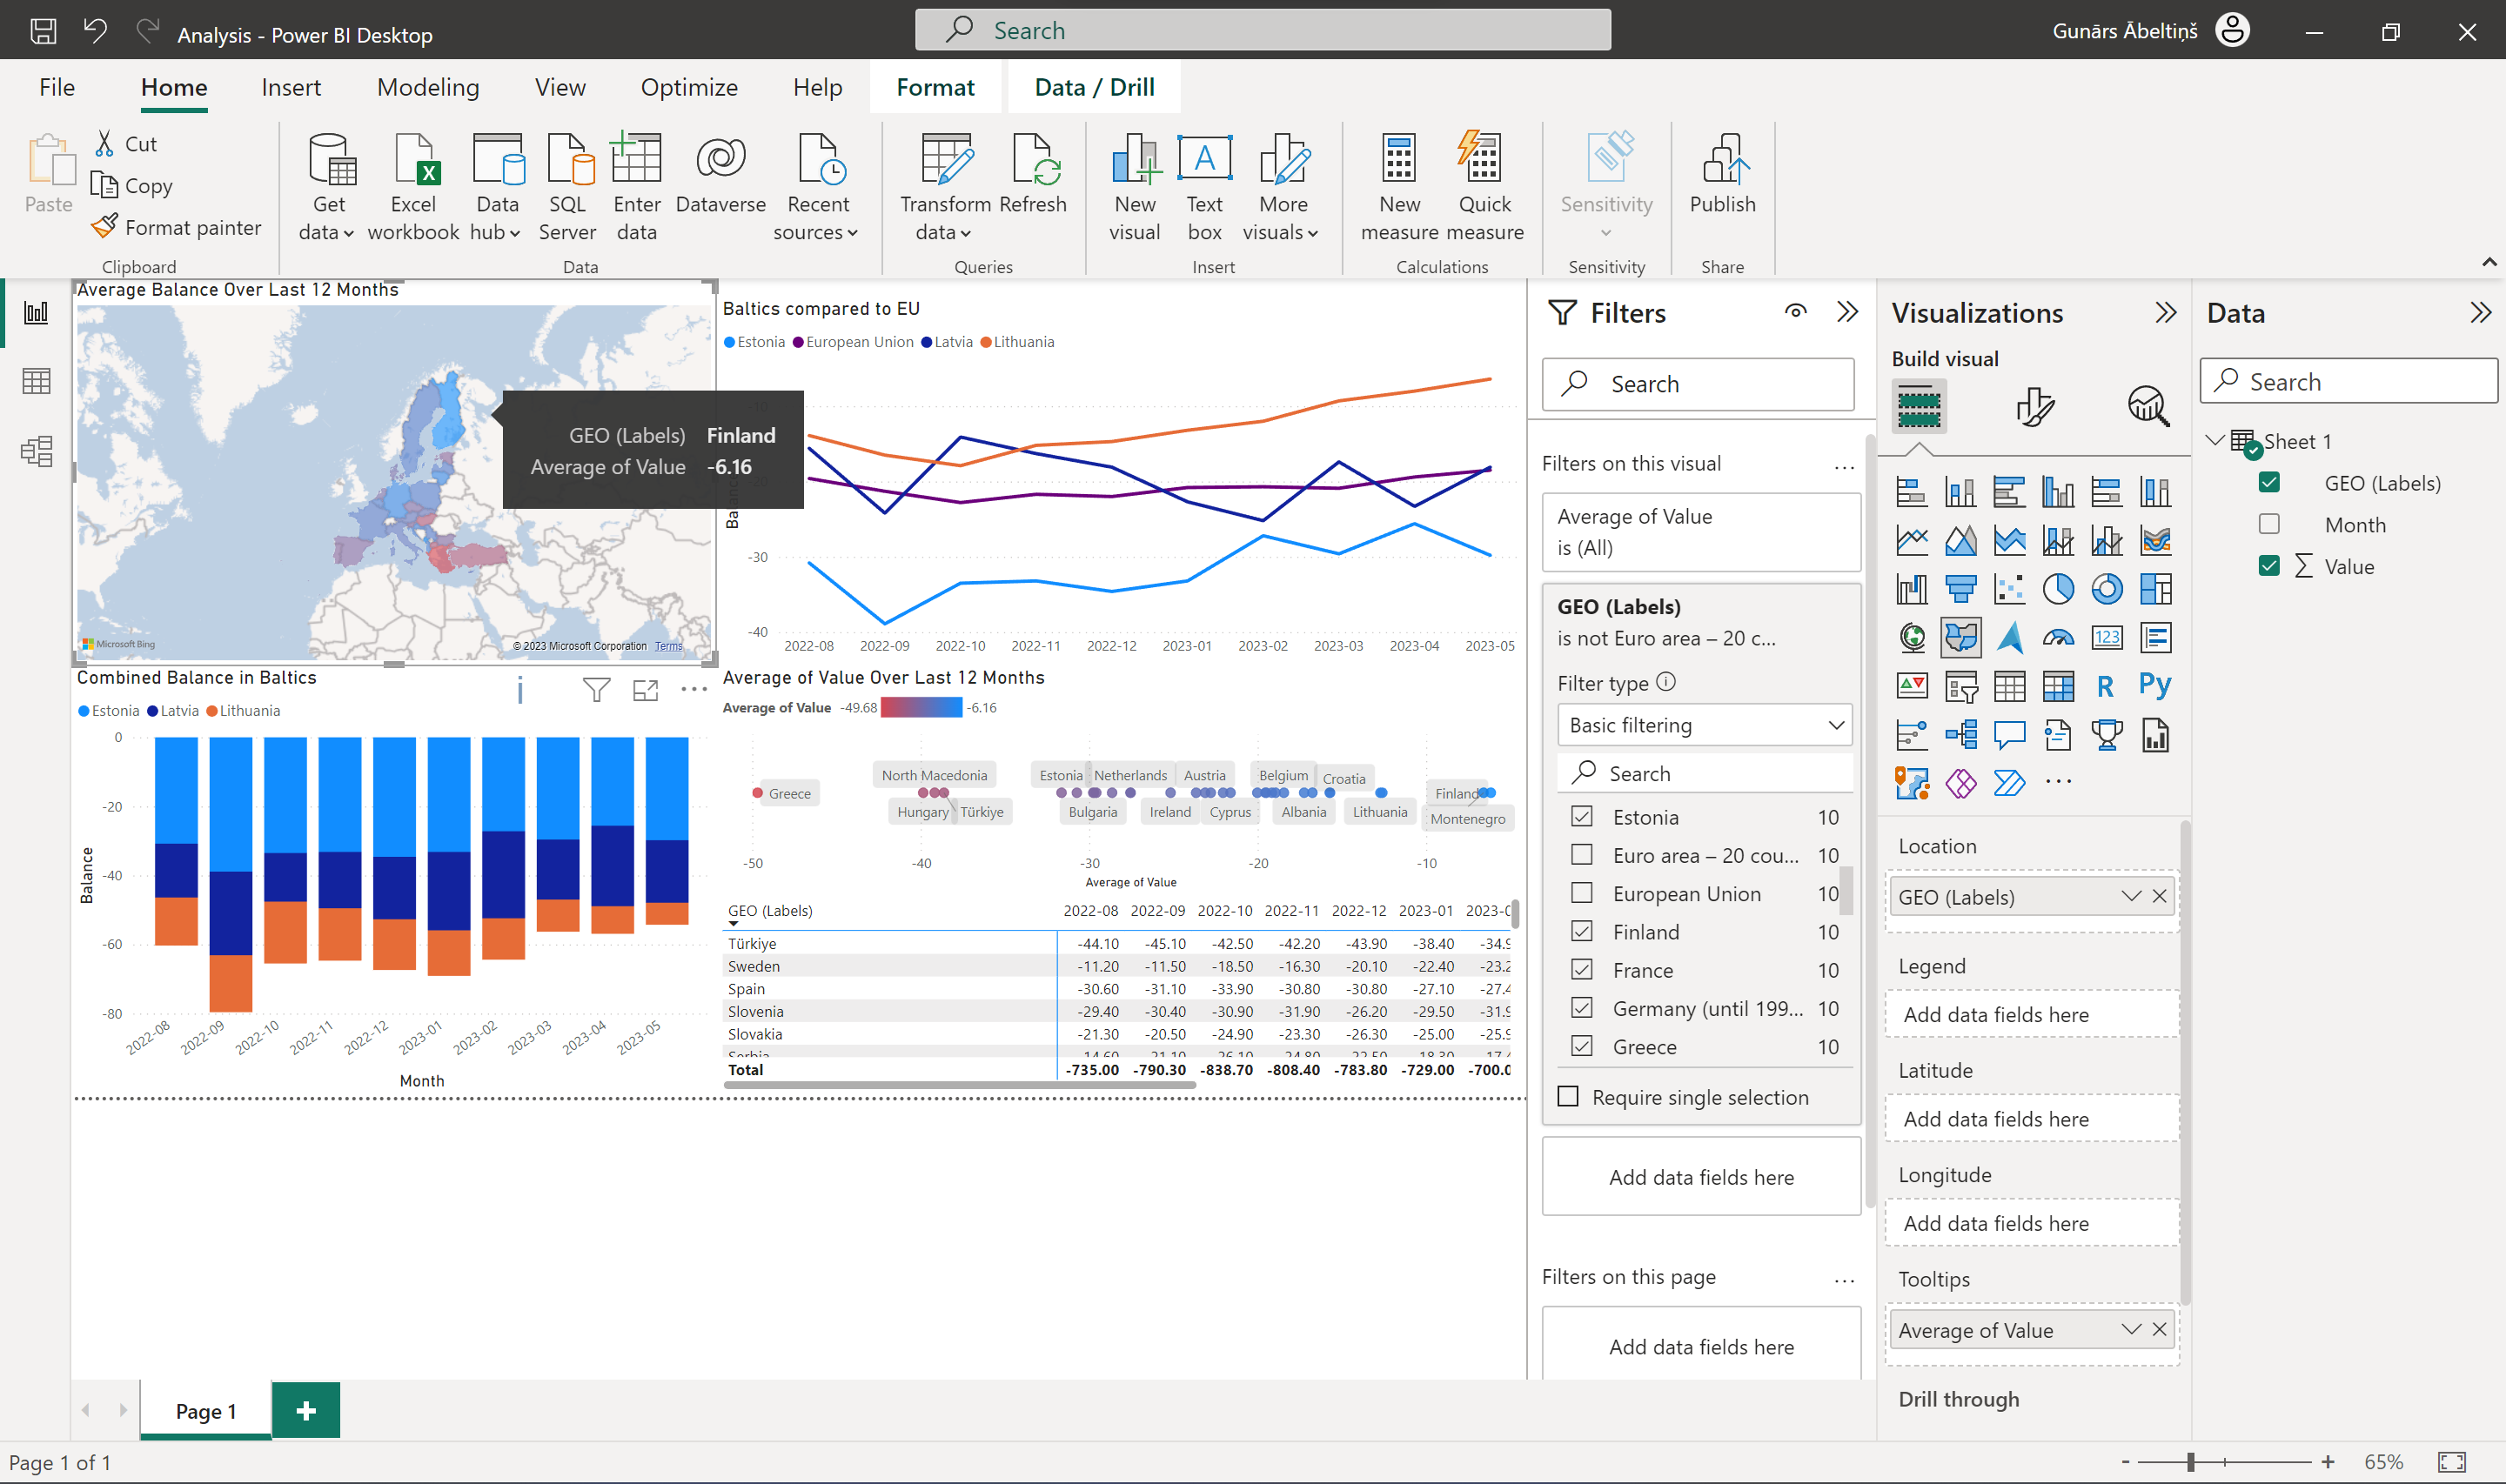
\includegraphics[width=0.9\textwidth, center]{Map}

Krāsa ir atkarīga no vidējas vērtibas pēdejo 12 mēnešu laika. Sarkanā krāsa apzīme sliktāku situāciju un zilā labāku.

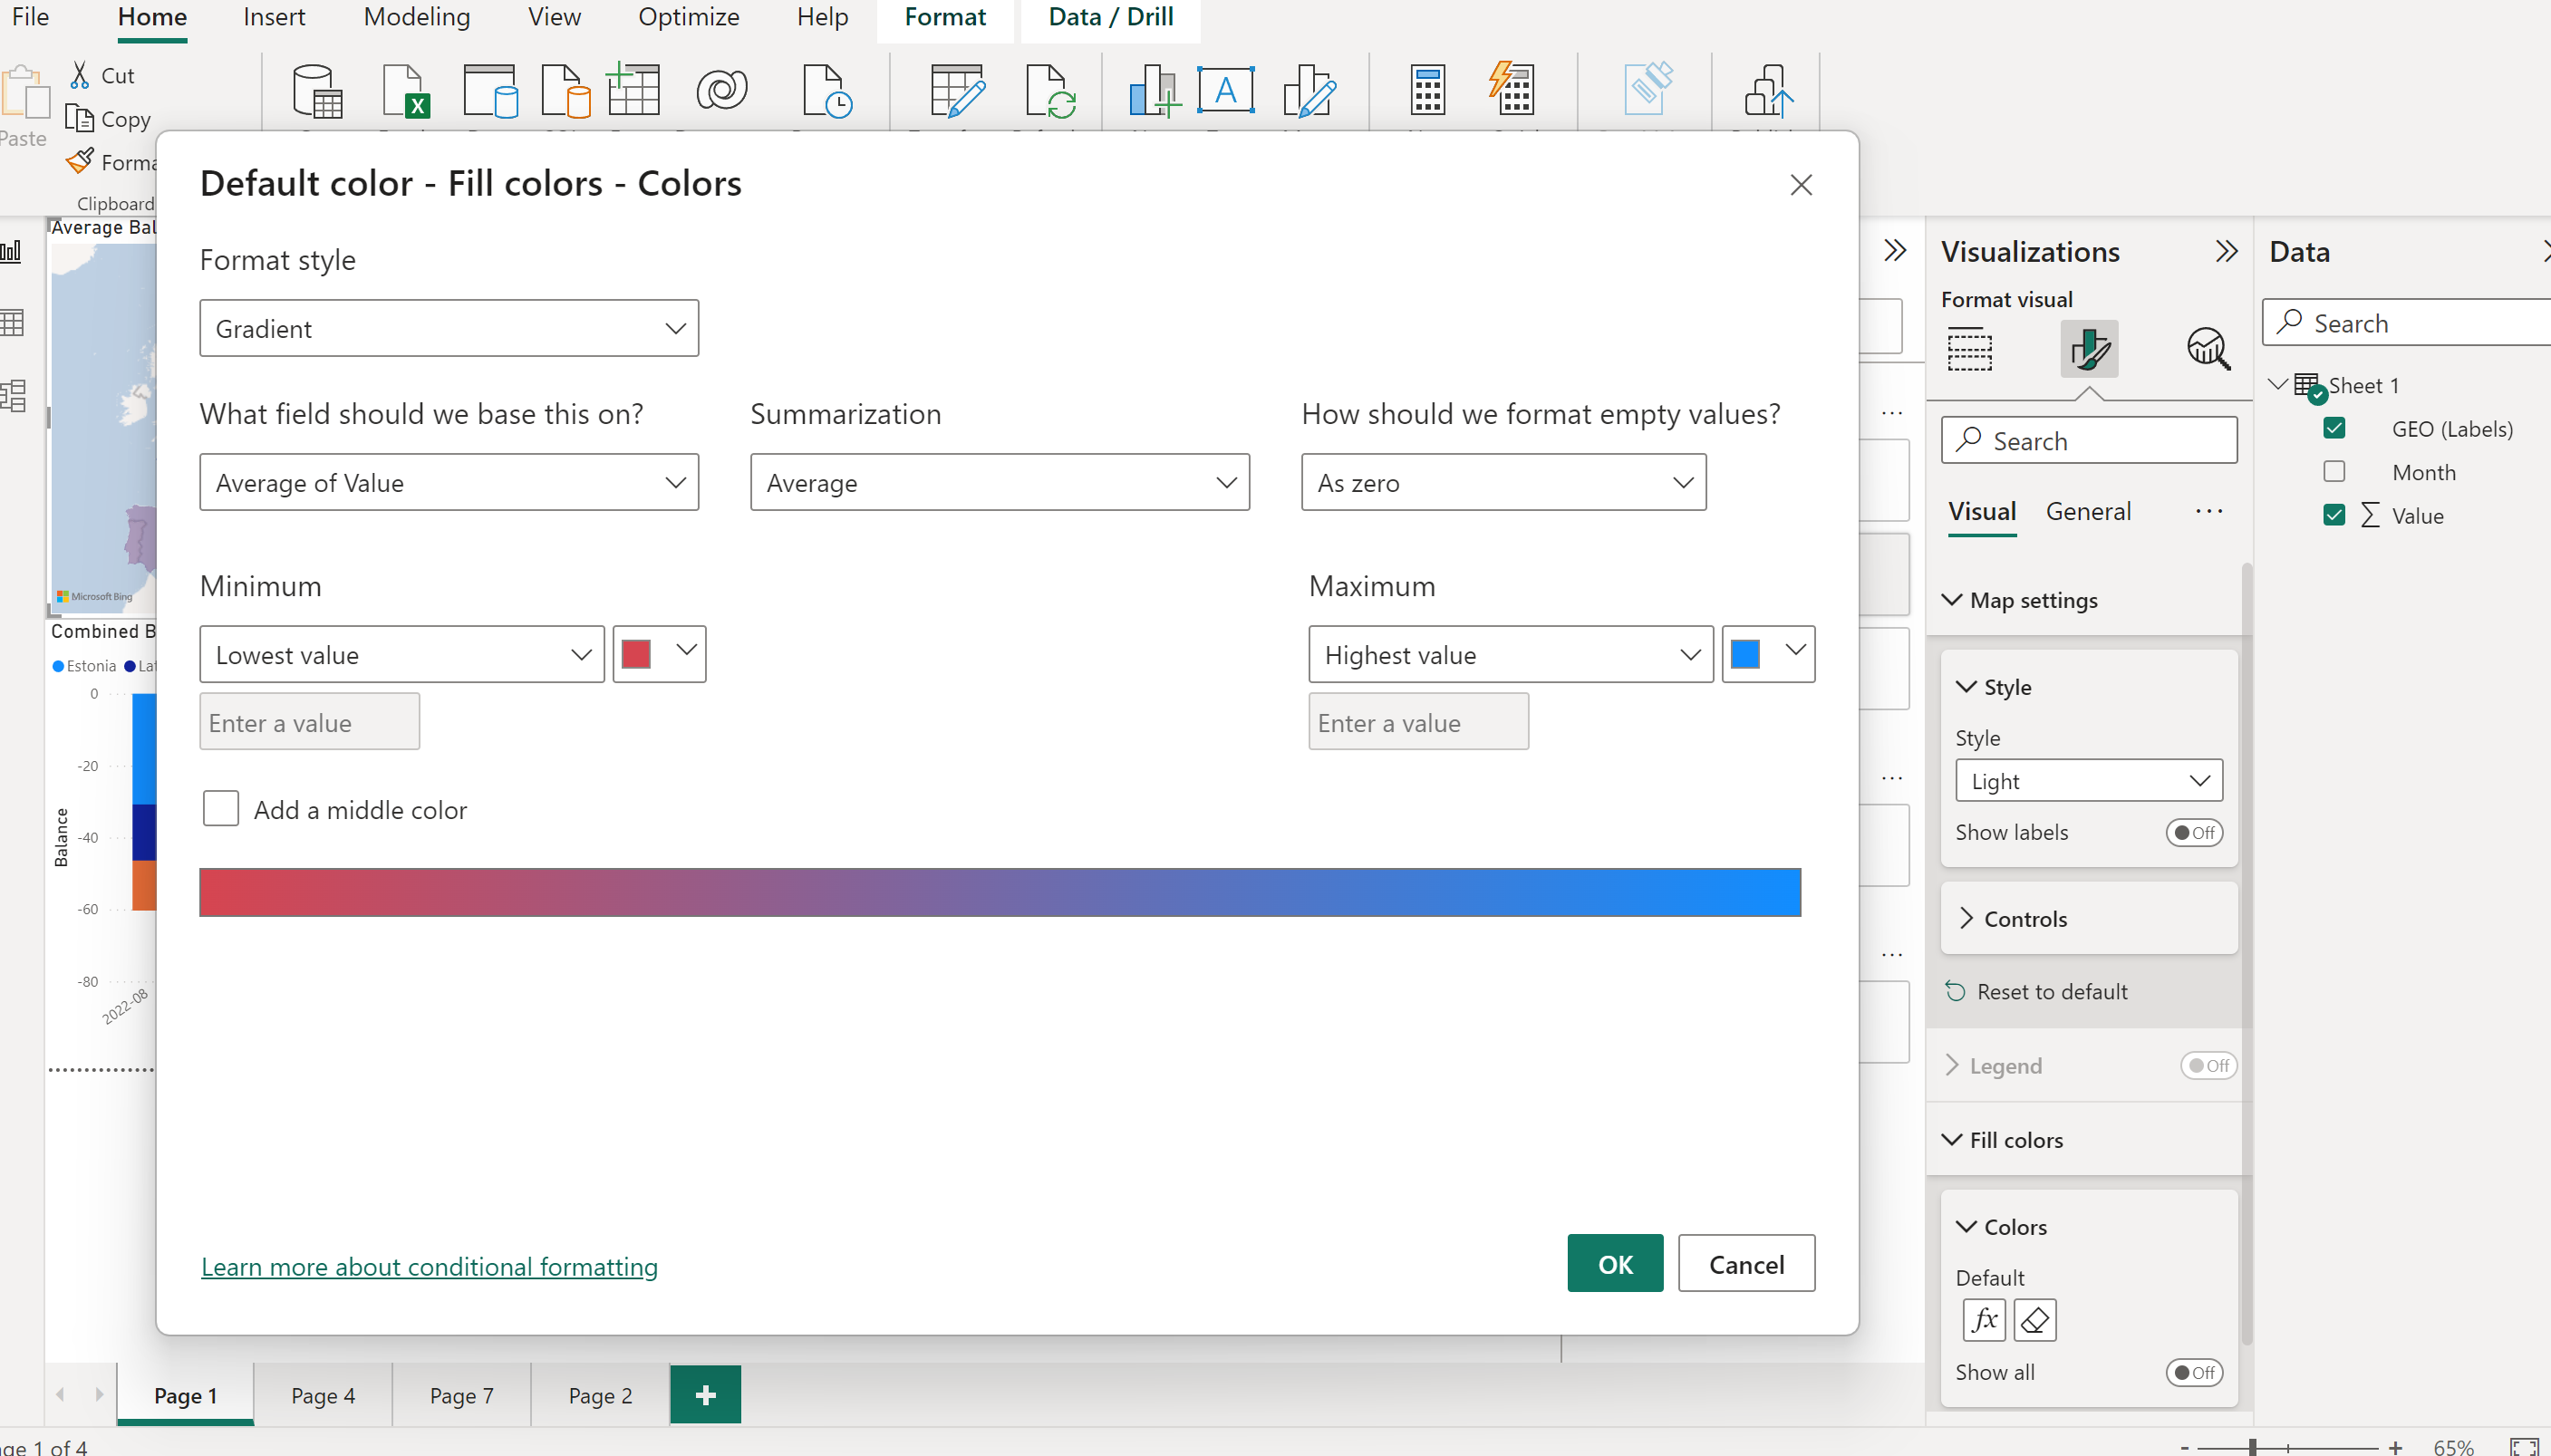
\includegraphics[width=0.9\textwidth, center]{Color}

\begin{itemize}
    \item Izmantotie datu lauki: GEO (Labels), Value
    \item Atrašanās vieta: GEO (Labels)
    \item Informācija: Value
    \item Filtri: Parādītas visas valstis izņemot "European Union" un "Euro area"
\end{itemize}


\subsubsection{Līniju diagramma}
Otrā diagramma, ko veidoju ir līniju diagramma, lai redzētu kā mainās situācija laika gaitā baltījas valstis. Pievienots arī ieropas vidējais rādītātjs, lai būtu ar ko salīdzināt.

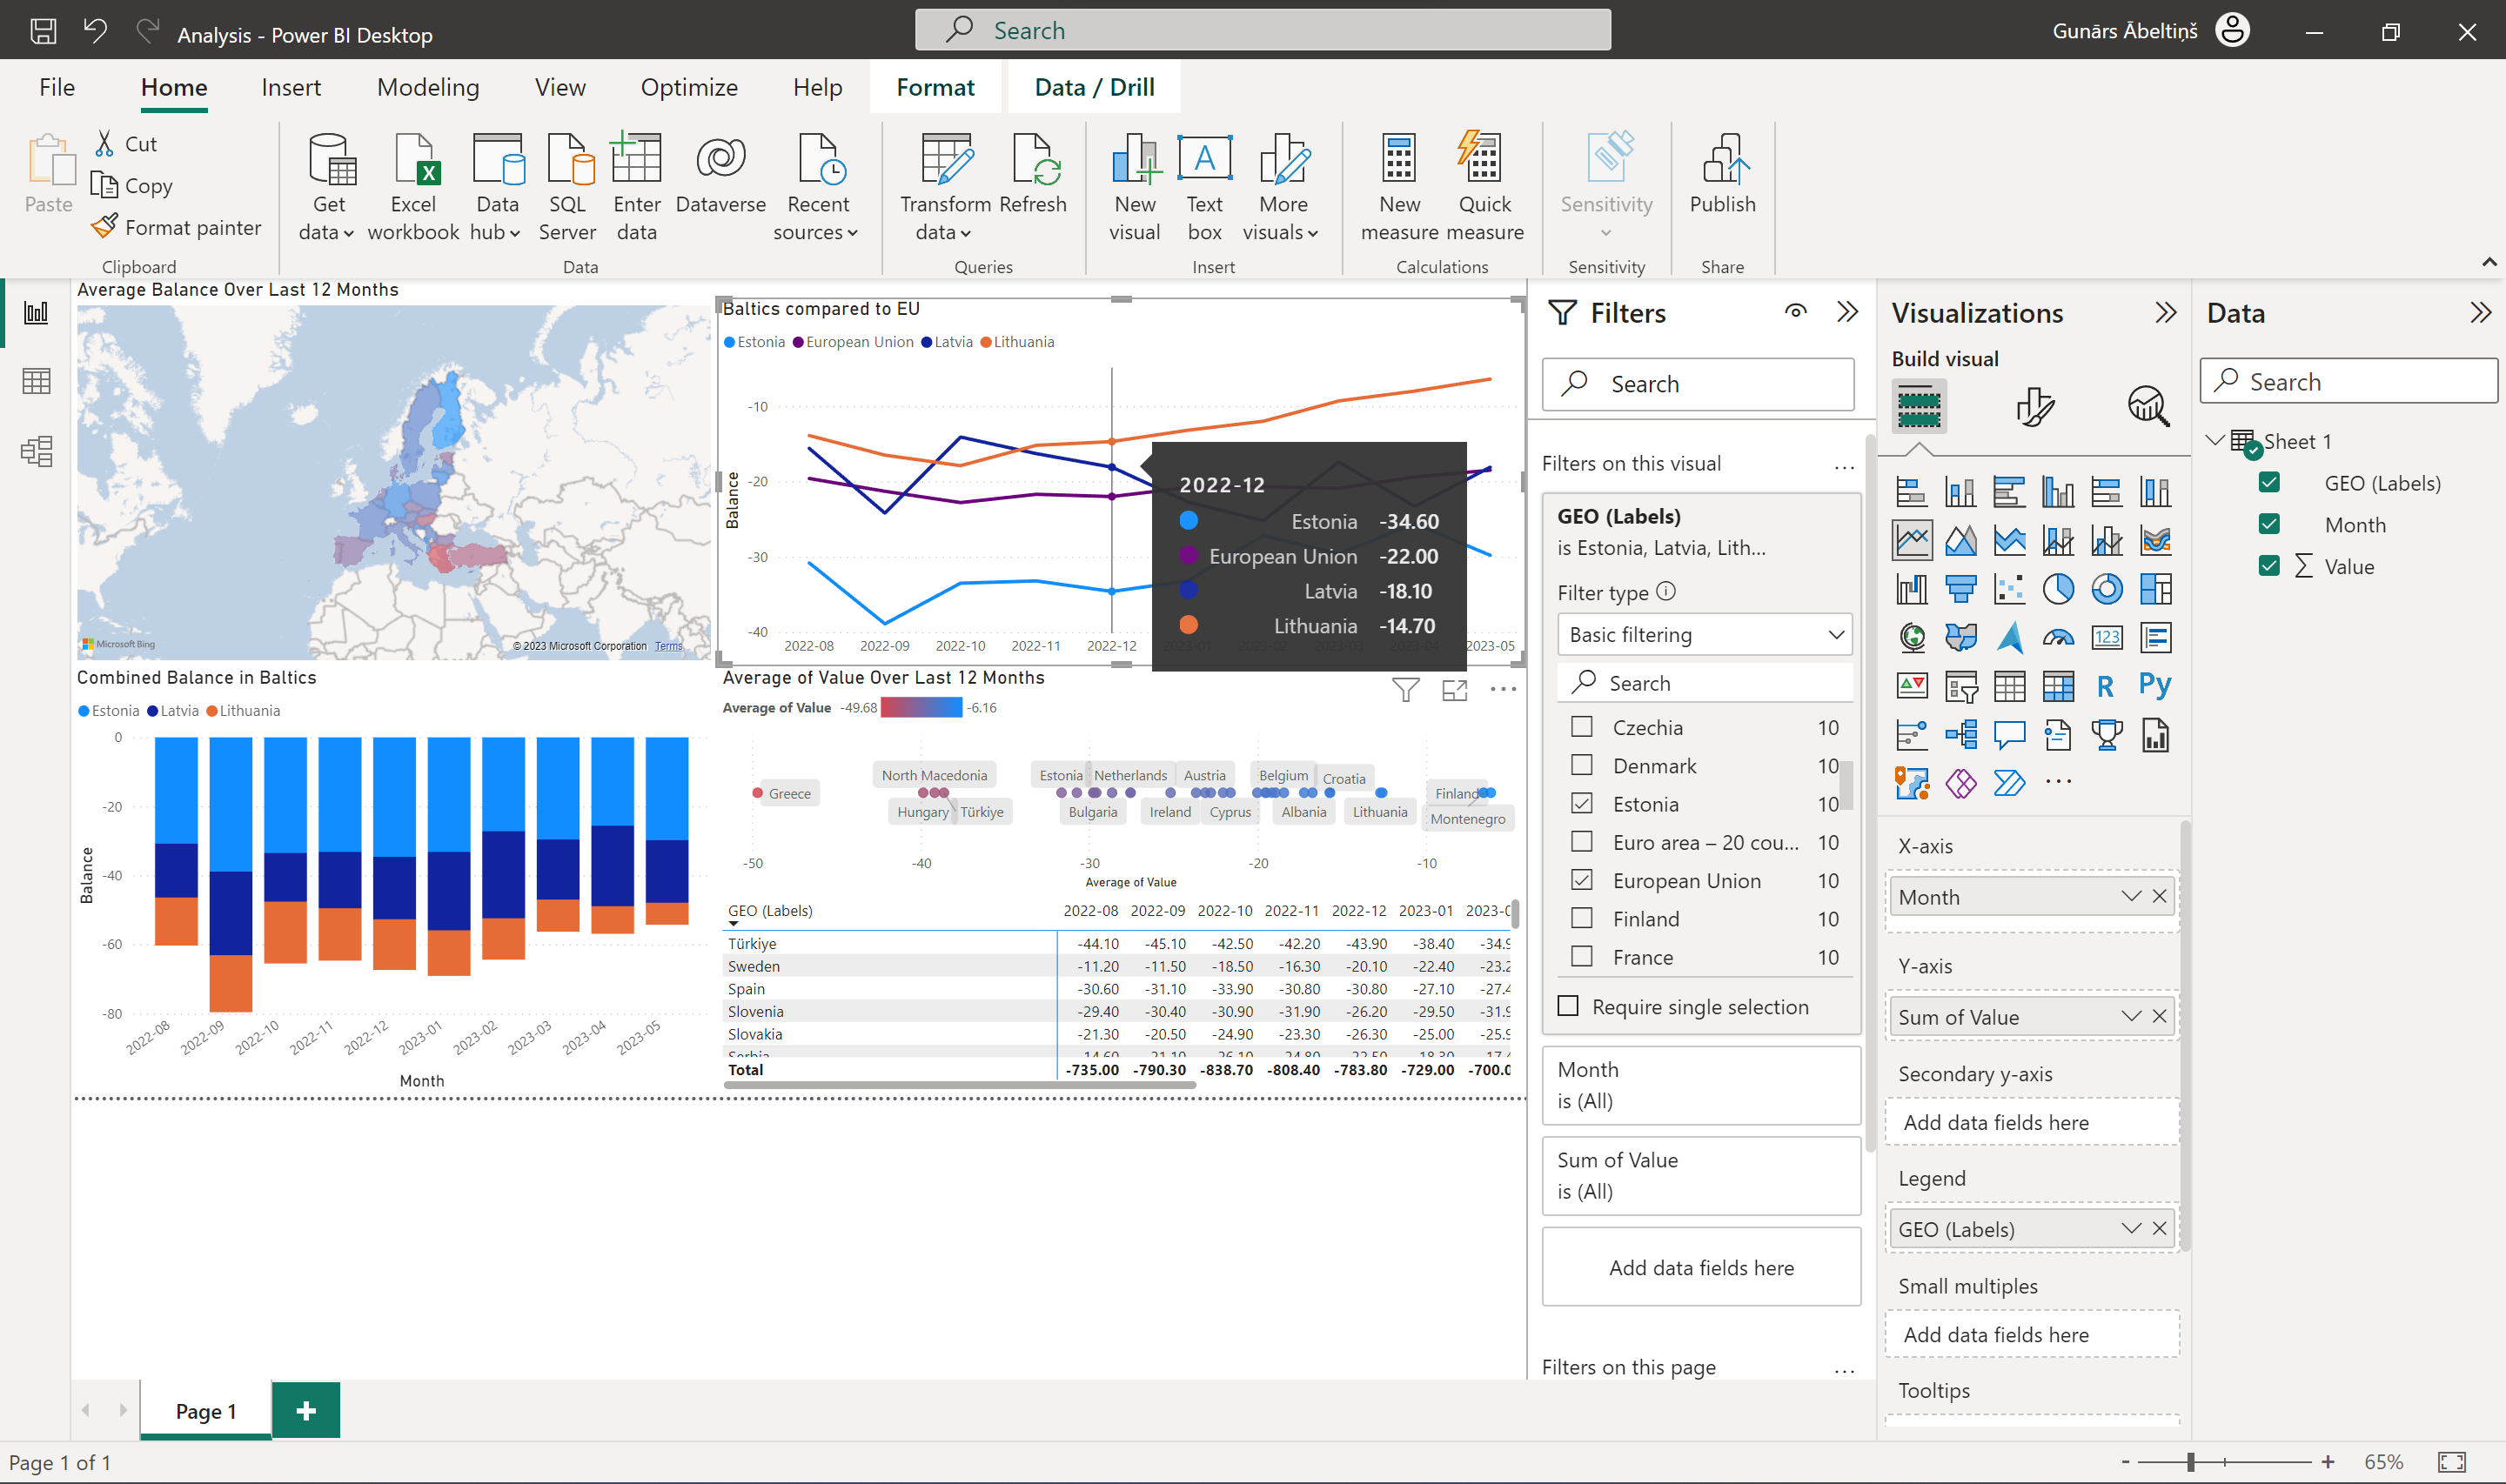
\includegraphics[width=0.9\textwidth, center]{Line}

\begin{itemize}
    \item Izmantotie datu lauki: GEO (Labels), Month, Value
    \item X ass: Month
    \item Y ass: Sum of Value
    \item Leģena: GEO (Labels)
    \item Filtri: Tiek pārādītas tikai baltijas valstis un eropas savienības vidējais
    \item Kārtošana: Hronoloģiski
\end{itemize}


\subsubsection{Saliktā kolonu diagramma}
Treša diagrama dot informāciju ka baltijas valstu rādītāji izskatās apvienoti kopā.

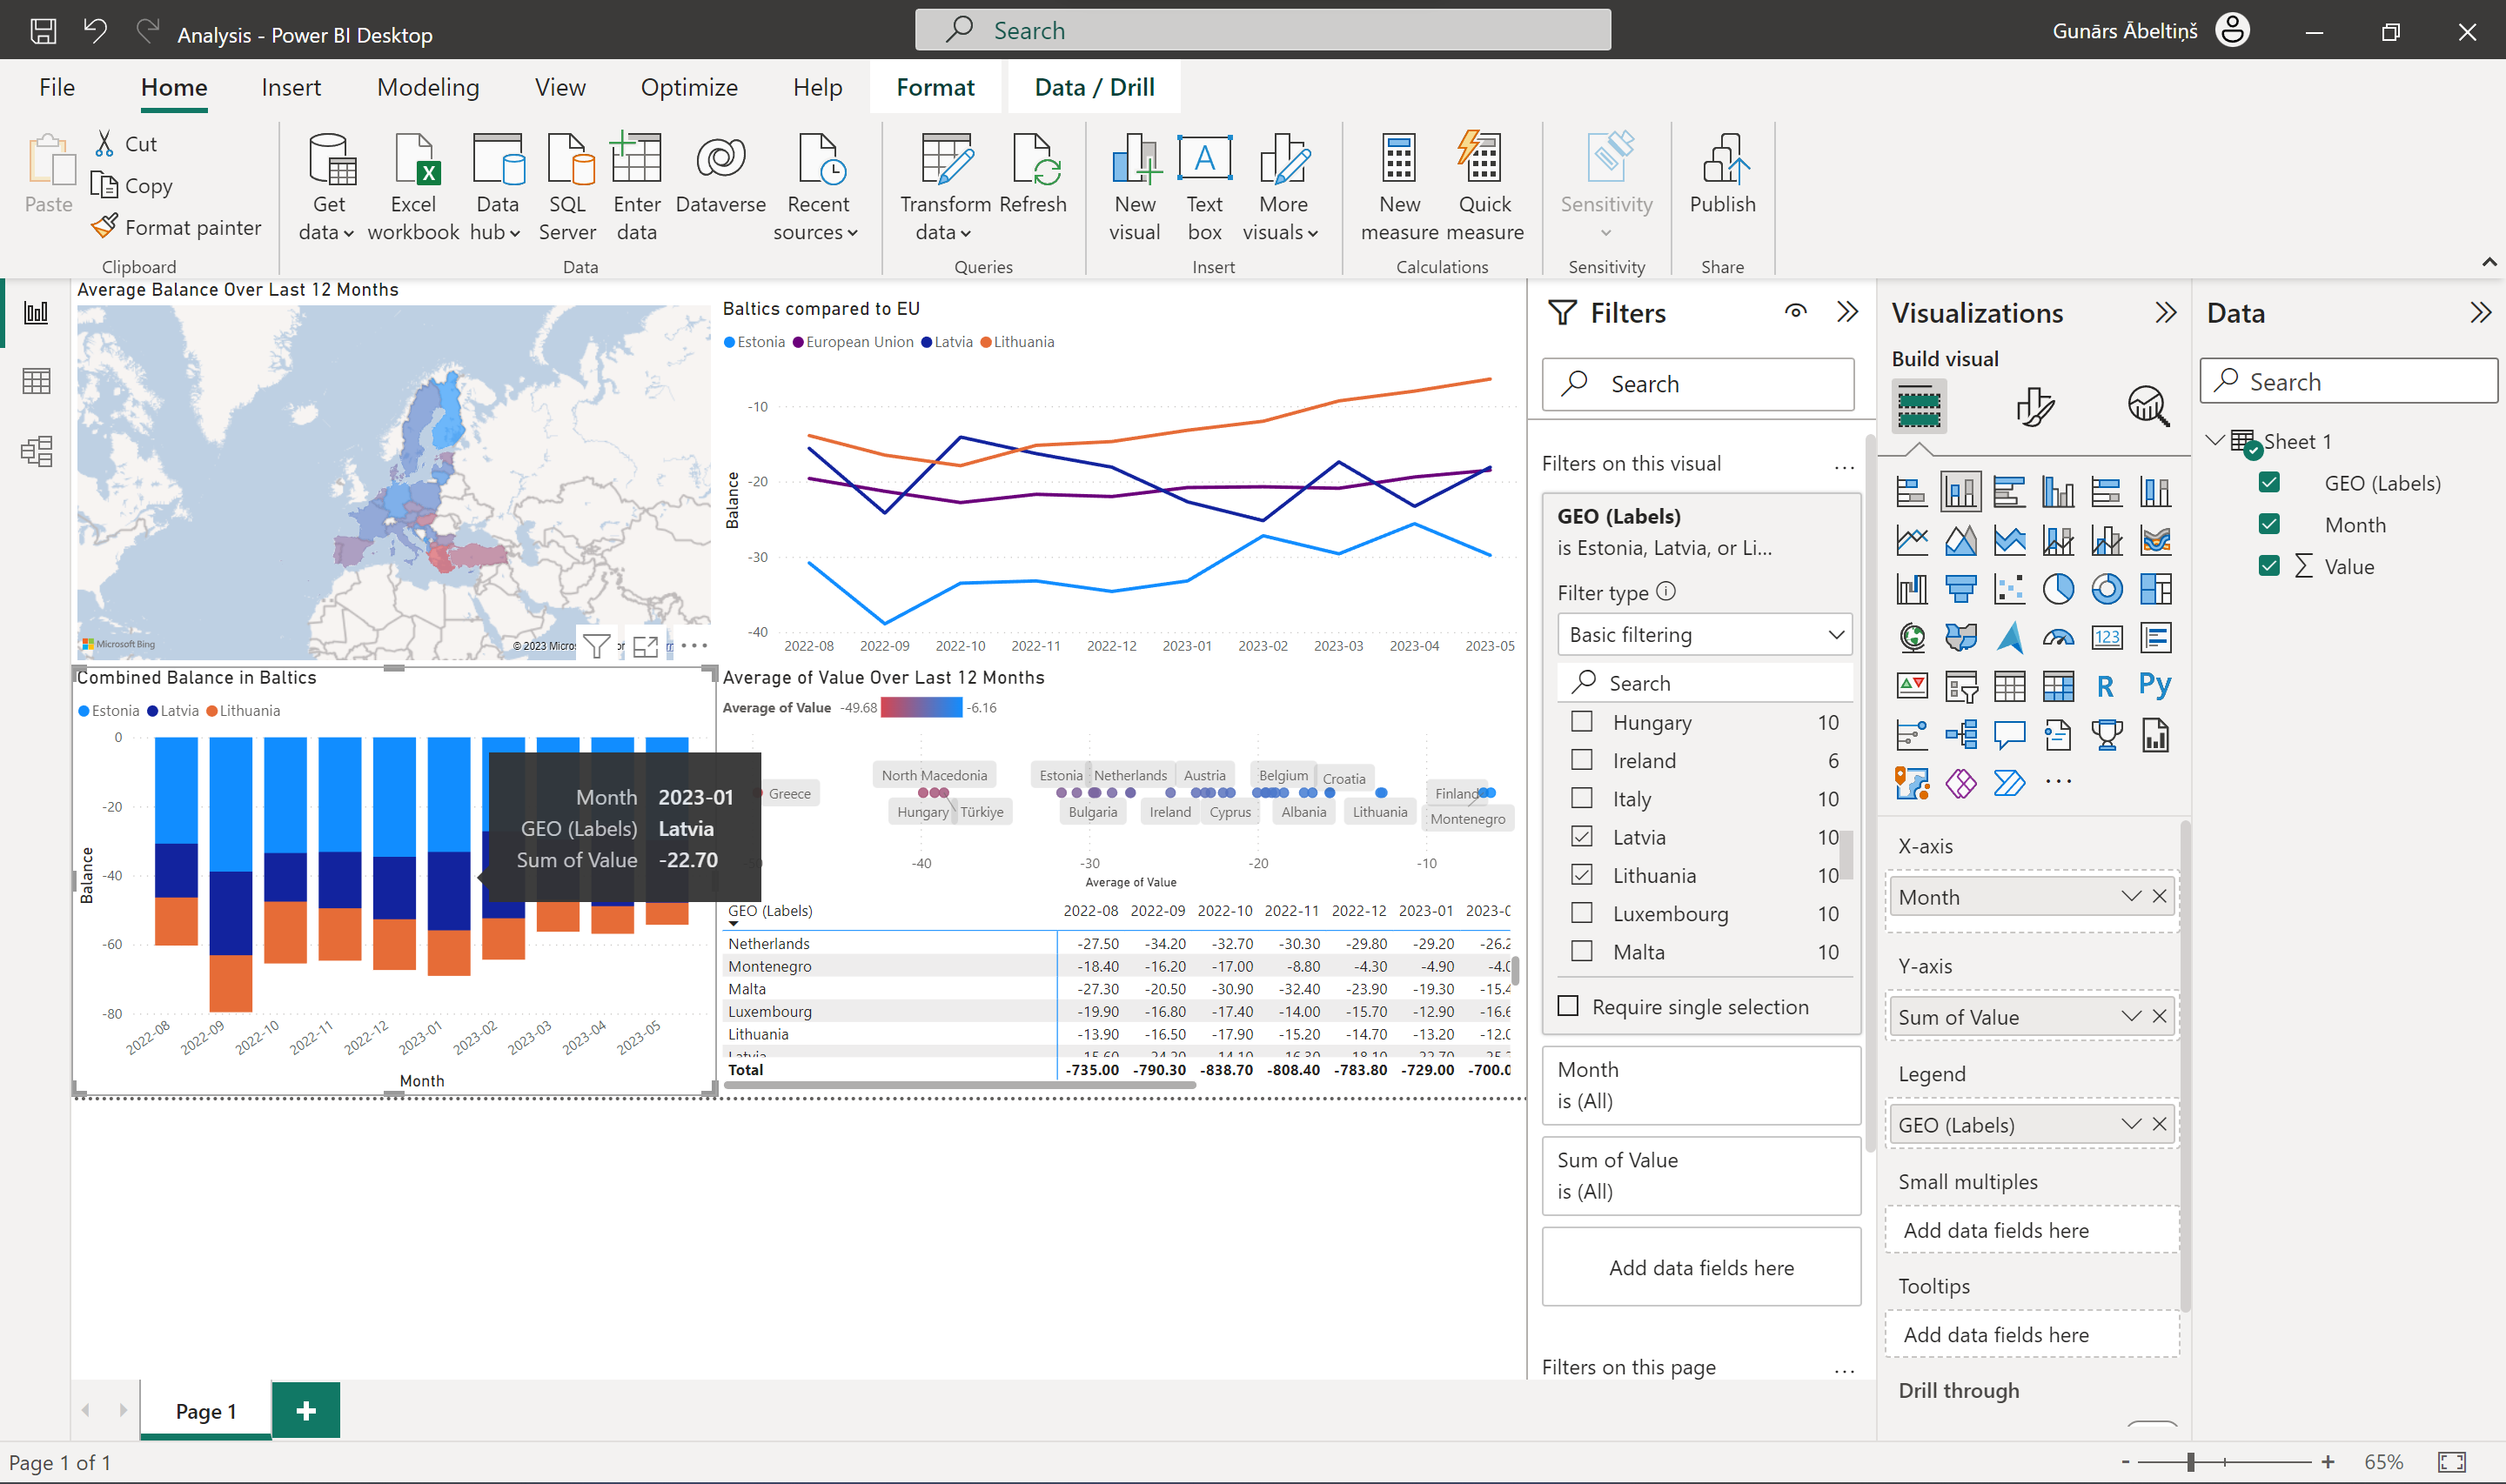
\includegraphics[width=0.9\textwidth, center]{Column}

\begin{itemize}
\item Izmantotie datu lauki: GEO (Labels), Month, Value
\item X ass: Month
\item Y ass: Sum of Value
\item Leģena: GEO (Labels)
\item Filtri: Tiek pārādītas tikai baltijas valstis
\item Kārtošana: Hronoloģiski
\end{itemize}


\subsubsection{Izkliedes diagramma}
Cetertā diagramma dod citu skatījumu uz visām valstīm kopā. Var uzskatāmāk redzēt kuras ir atšķirīgas no parējām.

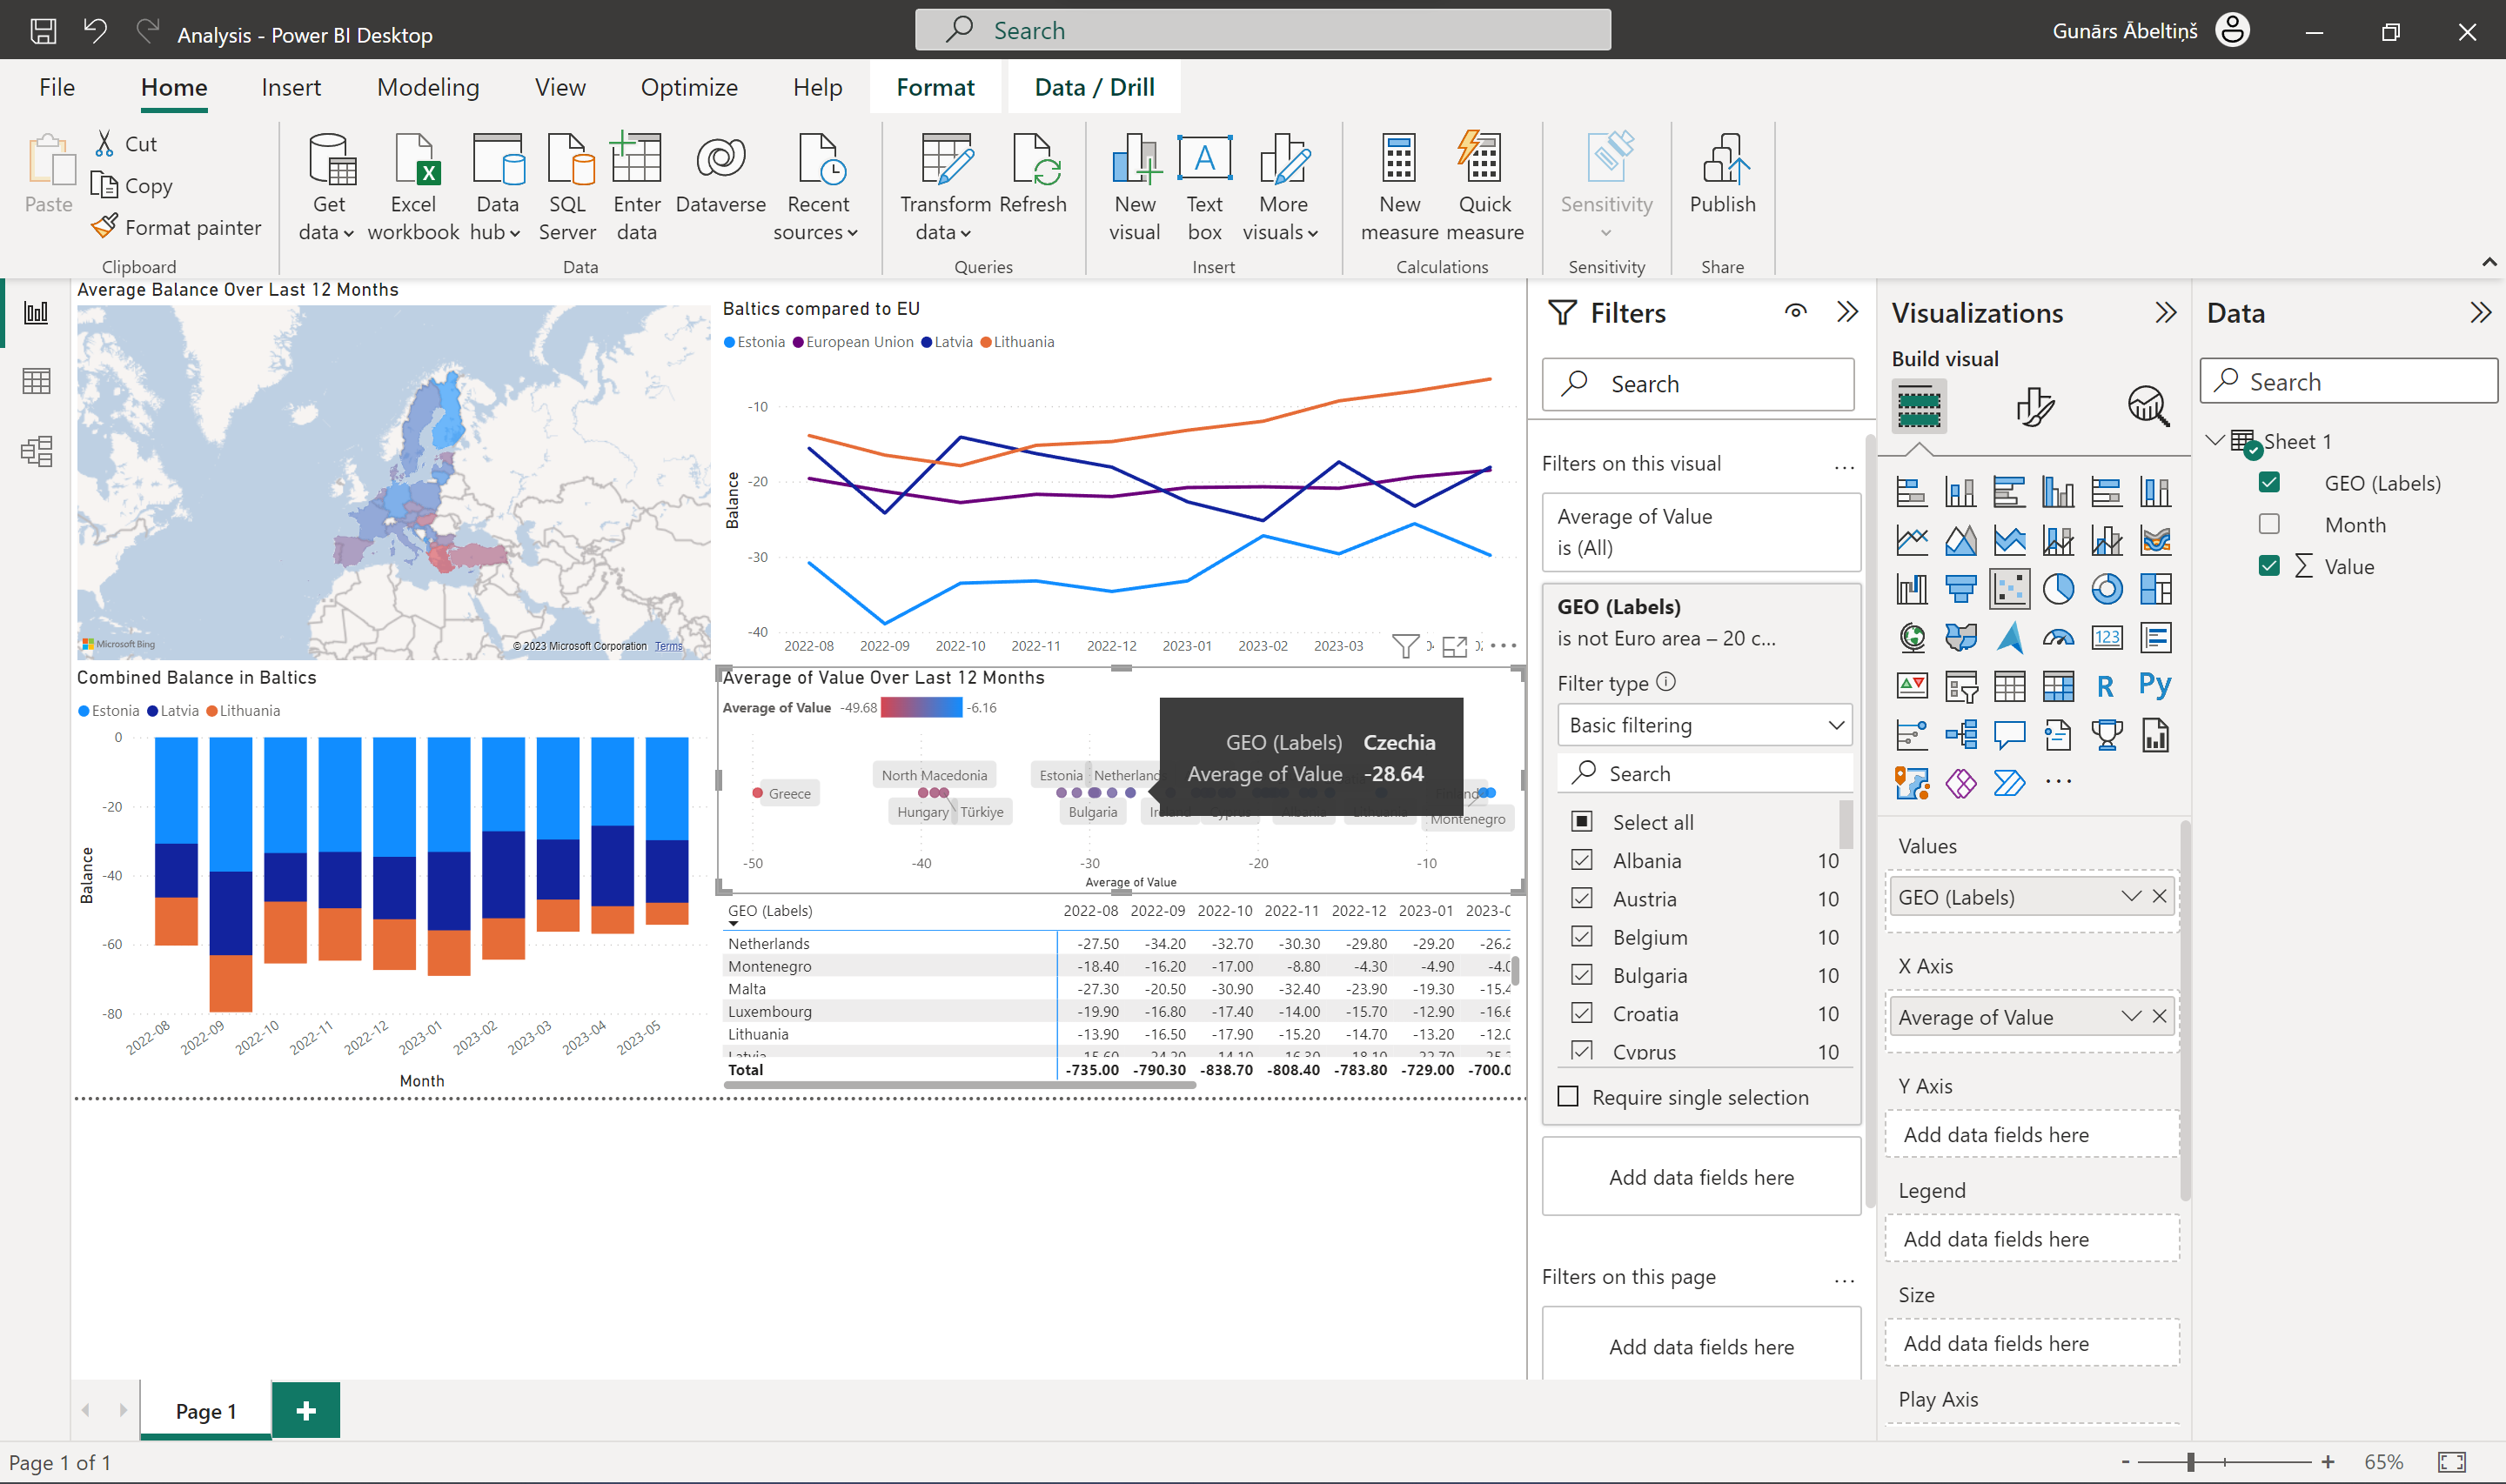
\includegraphics[width=0.9\textwidth, center]{Scatter}

\begin{itemize}
\item Izmantotie datu lauki: GEO (Labels) Value
\item Vērtības: GEO (Labels)
\item X ass: Average of Value
\end{itemize}

\subsubsection{Tabula}
Kā pēdējo pievienoju vienkāršu tabulu, ja nu lietotājam pašam gribas atrast kādu konkrētu valsti pēc vārda.

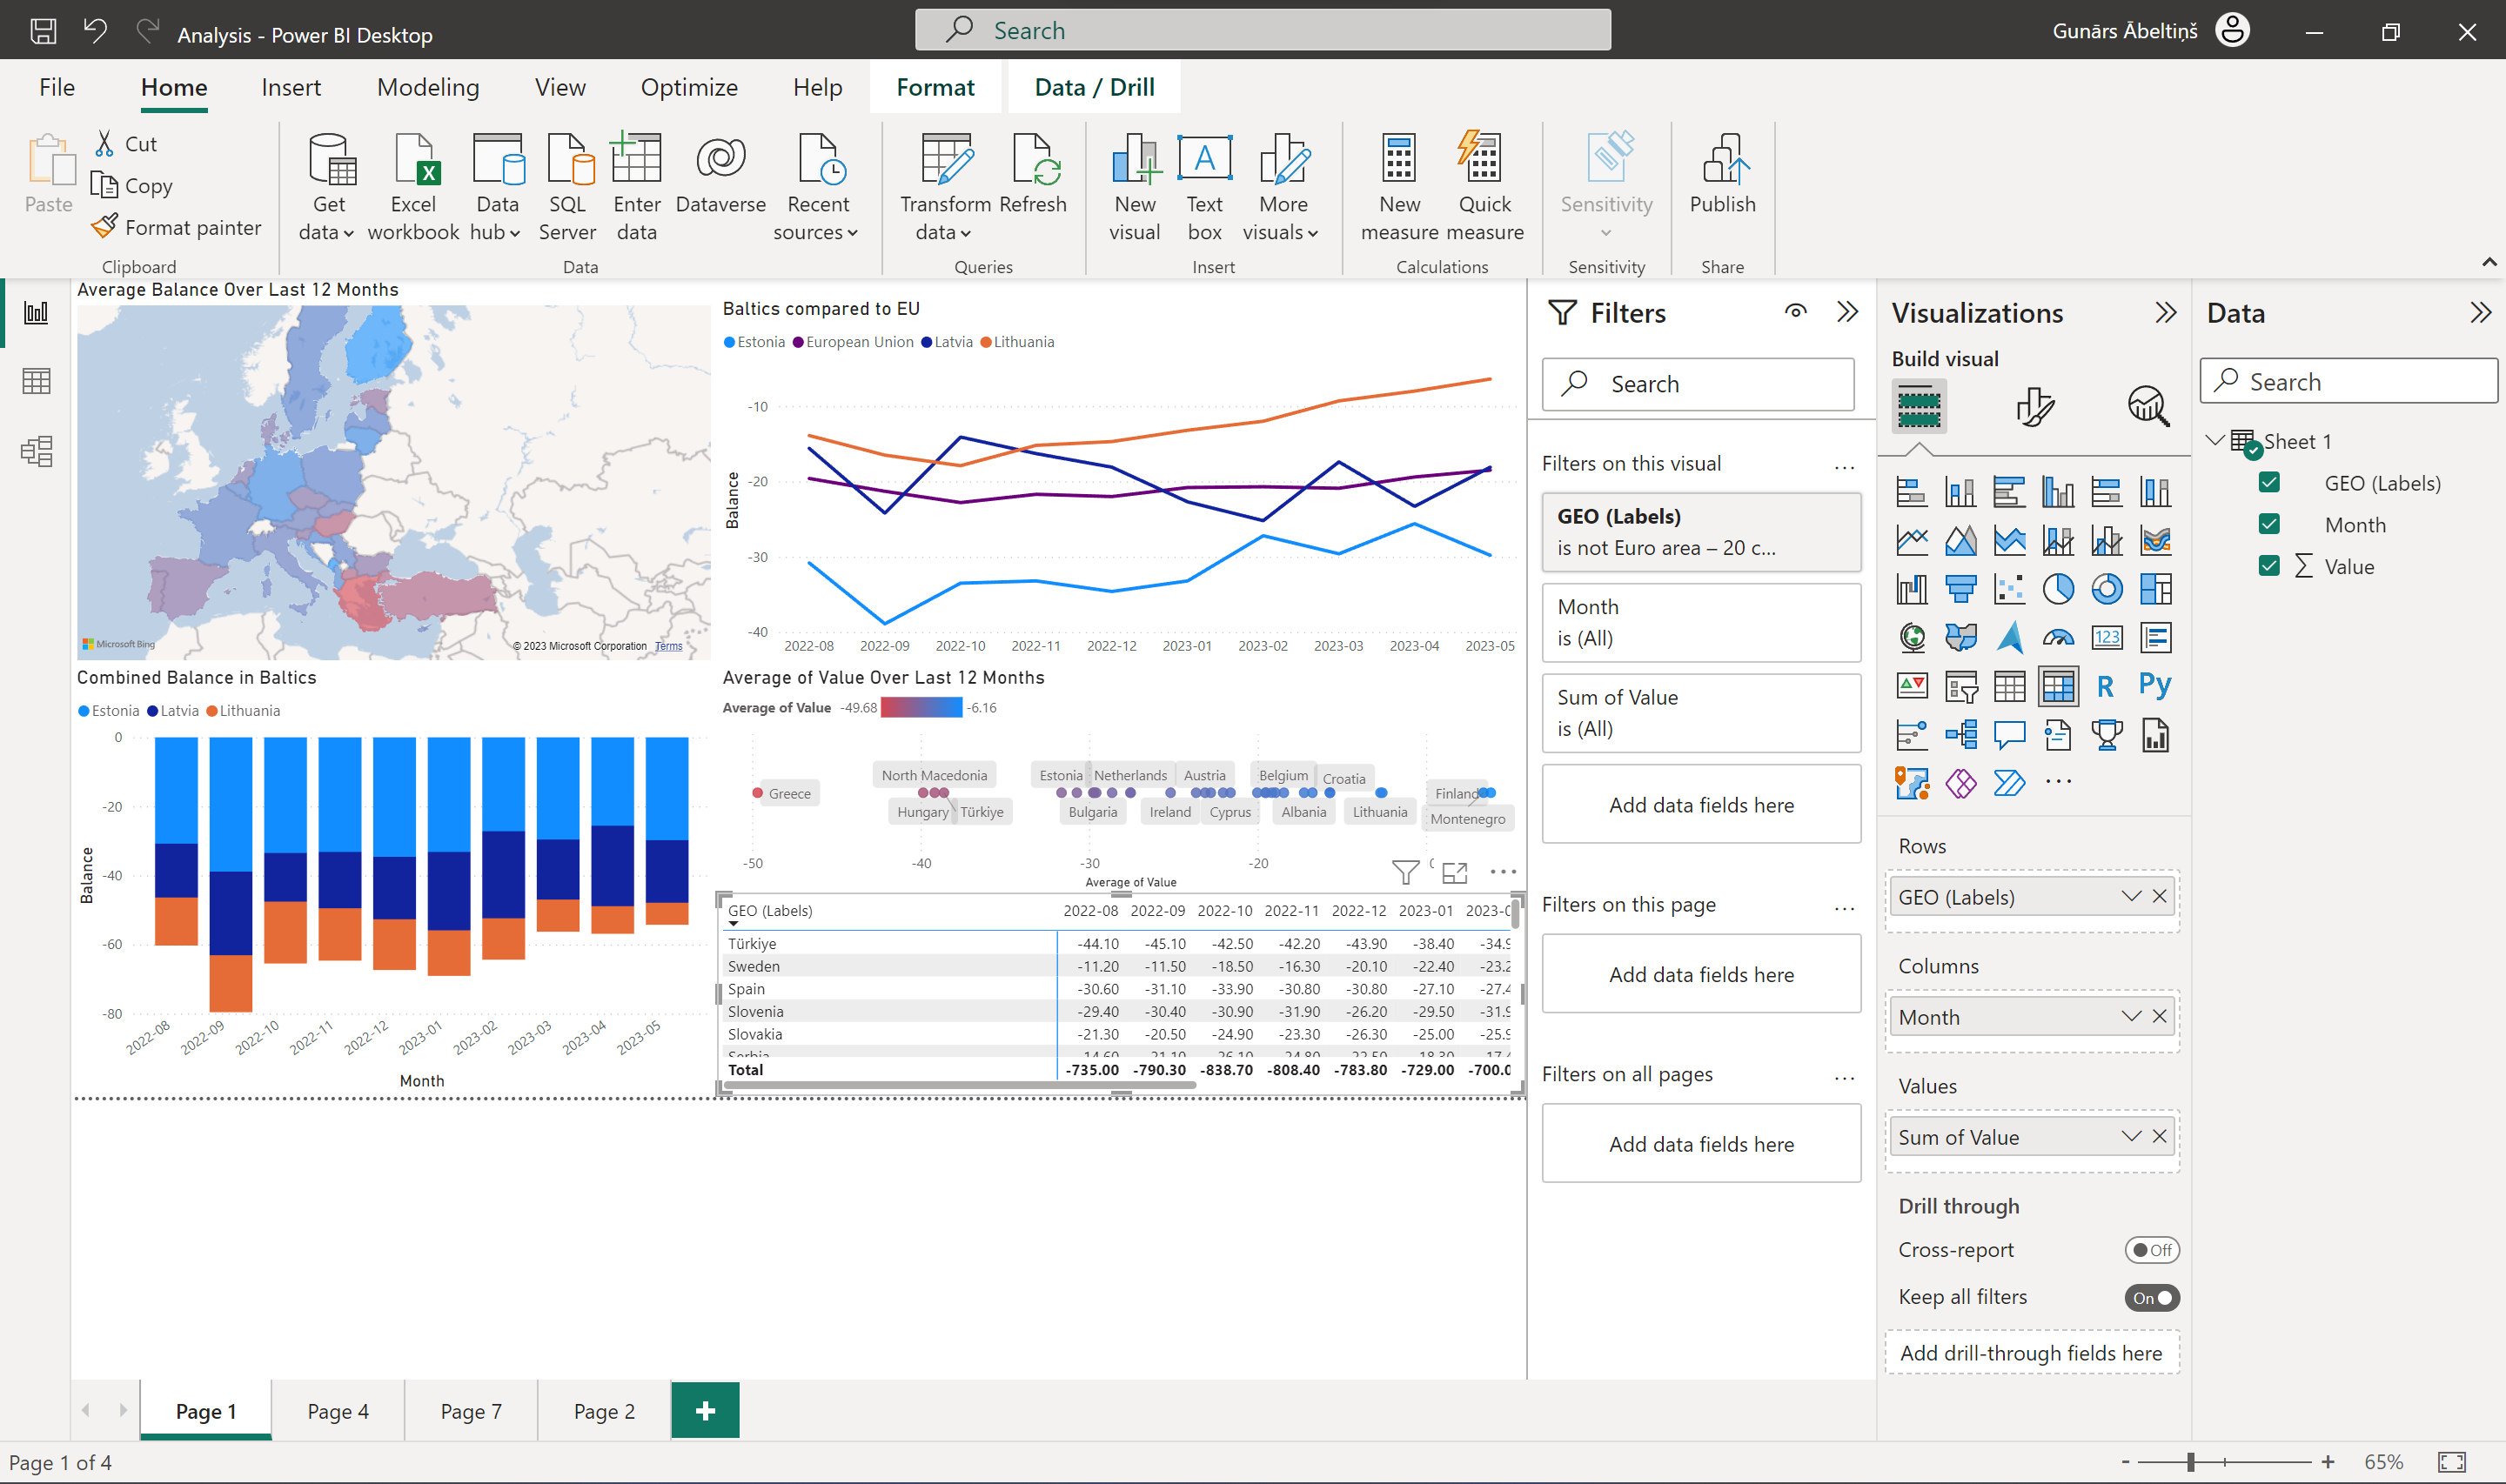
\includegraphics[width=0.9\textwidth, center]{Matrix}

\begin{itemize}
    \item Izmantotie datu lauki: GEO (Labels), Month, Value
    \item Rindas: GEO (Labels)
    \item Kolonas: Month
    \item Vērtibas: Sum of Value
    \item Kārtošana: Alfabēta secībā
\end{itemize}

\section{Gala rezultāts}

Kopumā tika iegūtas 5 atskaites, kas var palīdzēt izprast situāciju baltijas valstīs un eiropā.

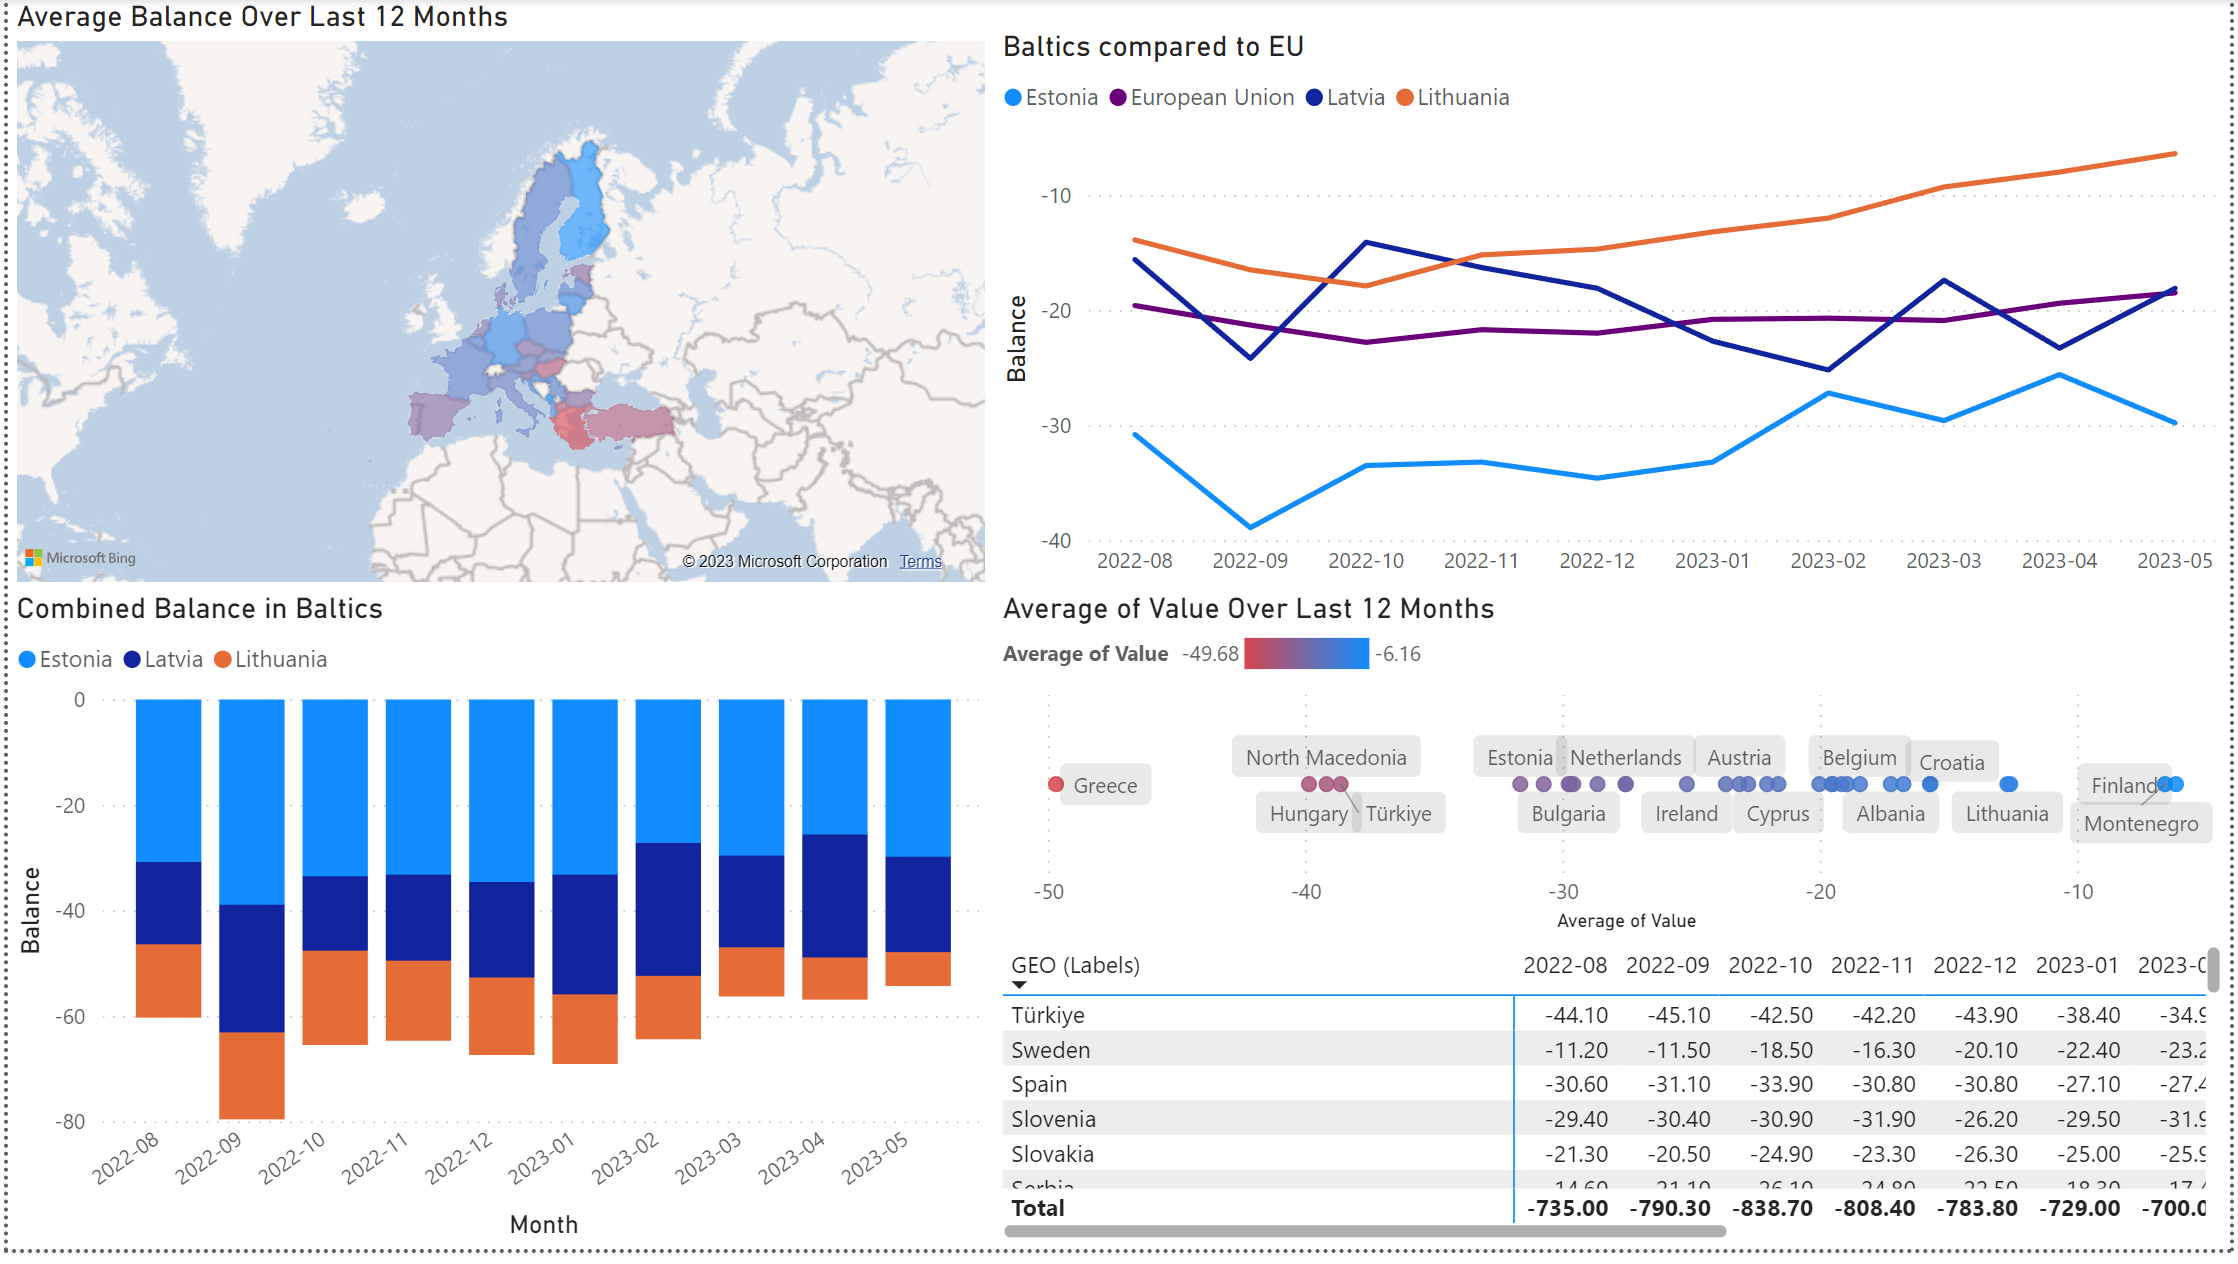
\includegraphics[width=0.9\textwidth, center]{Overview}

Ir iespējams atlasīt tikai vienu valsti, lai tiktu izcelta tikai tās informācija. To var izdarīt no baltijas valstu daigramām.

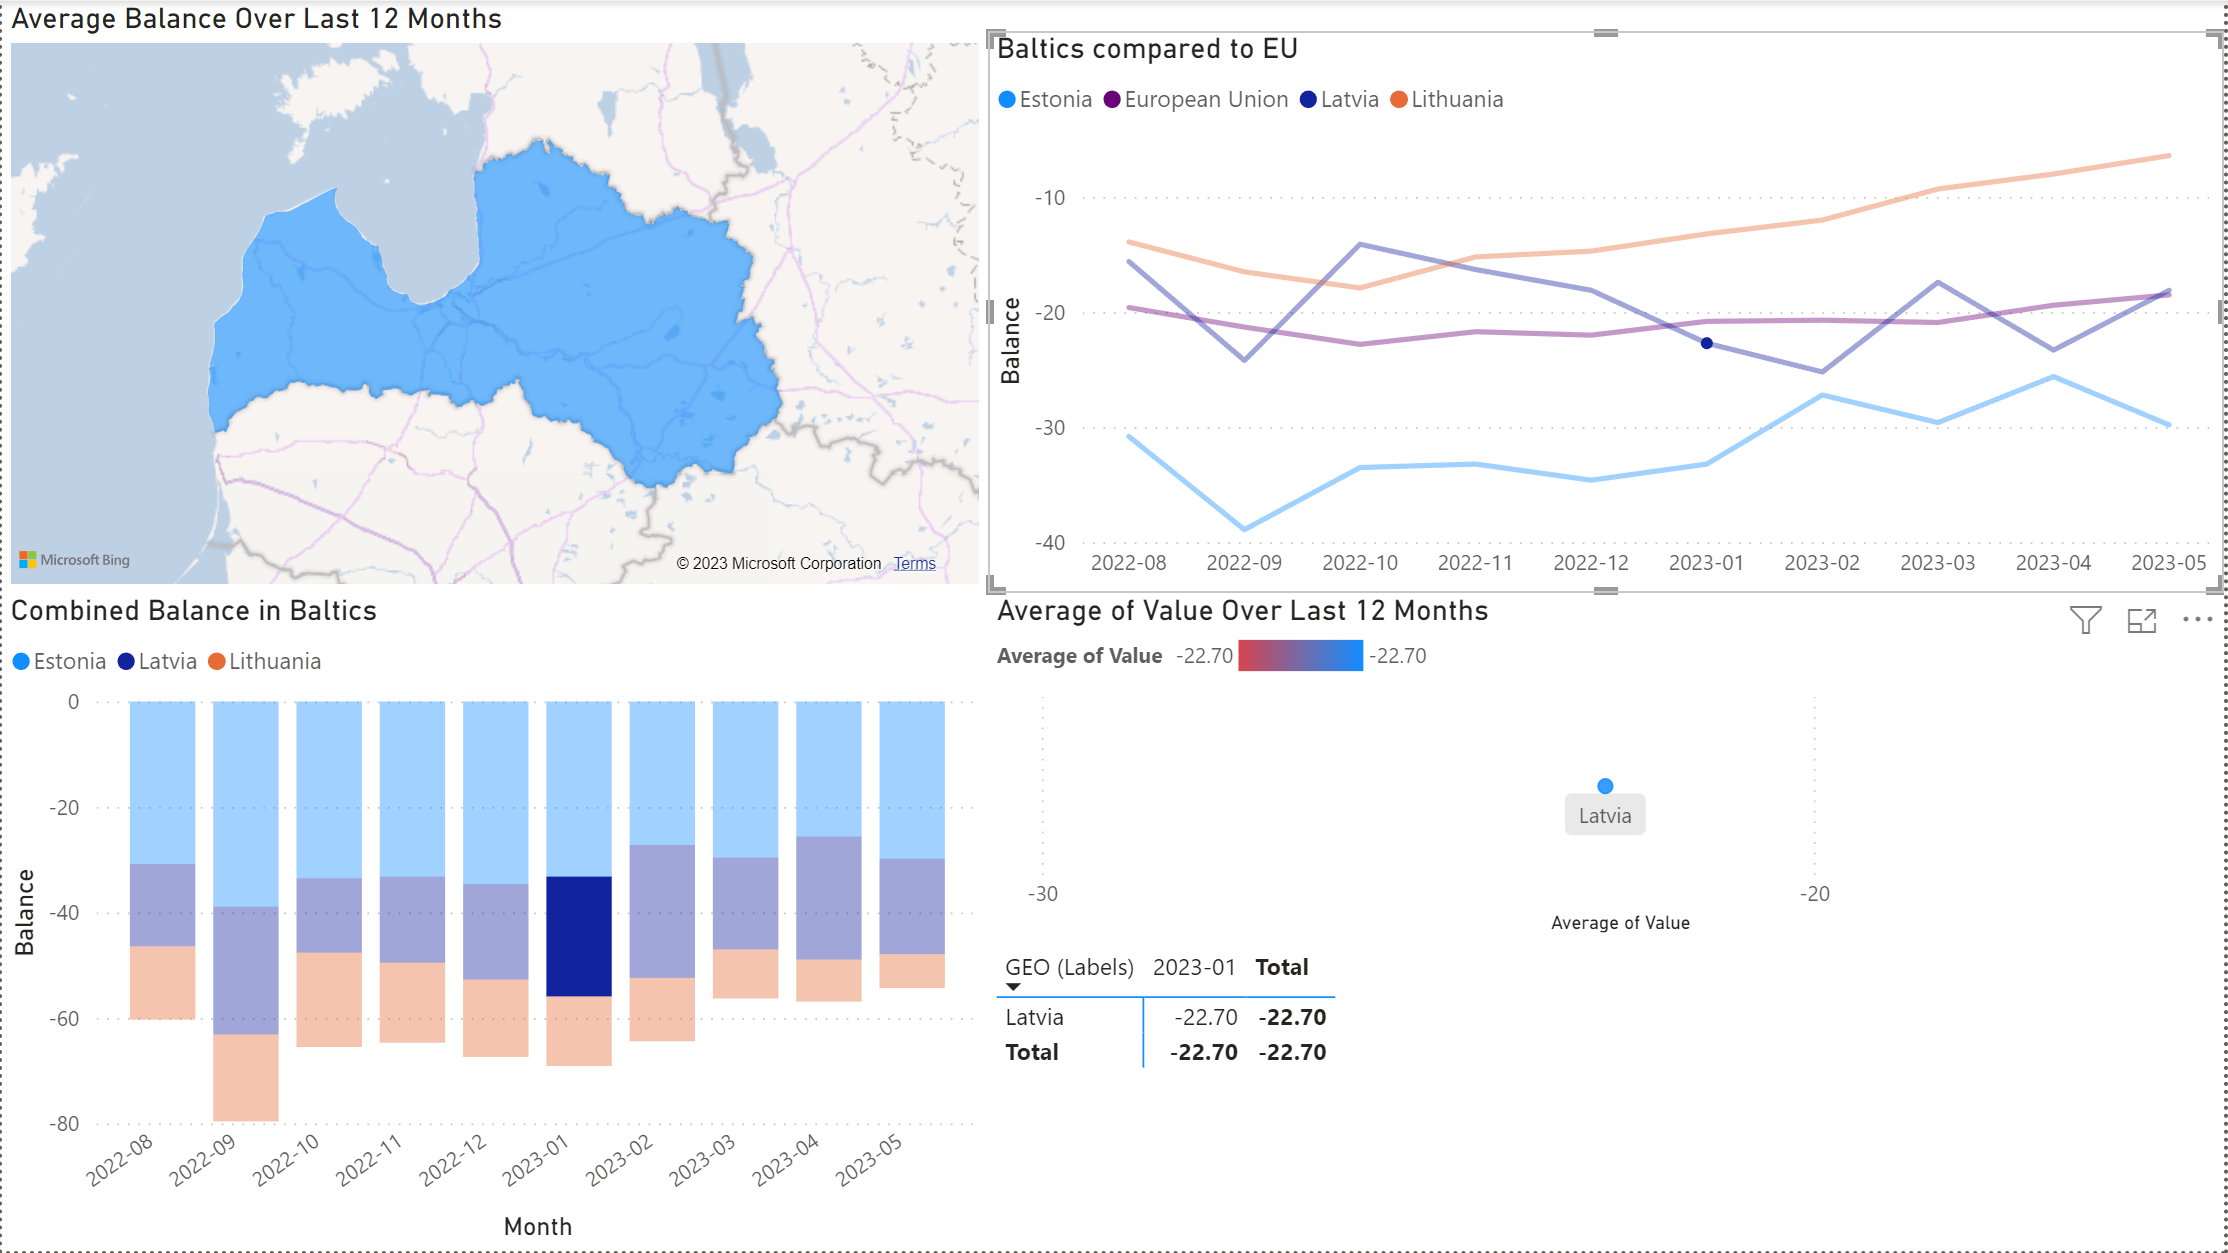
\includegraphics[width=0.9\textwidth, center]{Latvia}

Un ari no parējām diagramām ar visām valstīm.

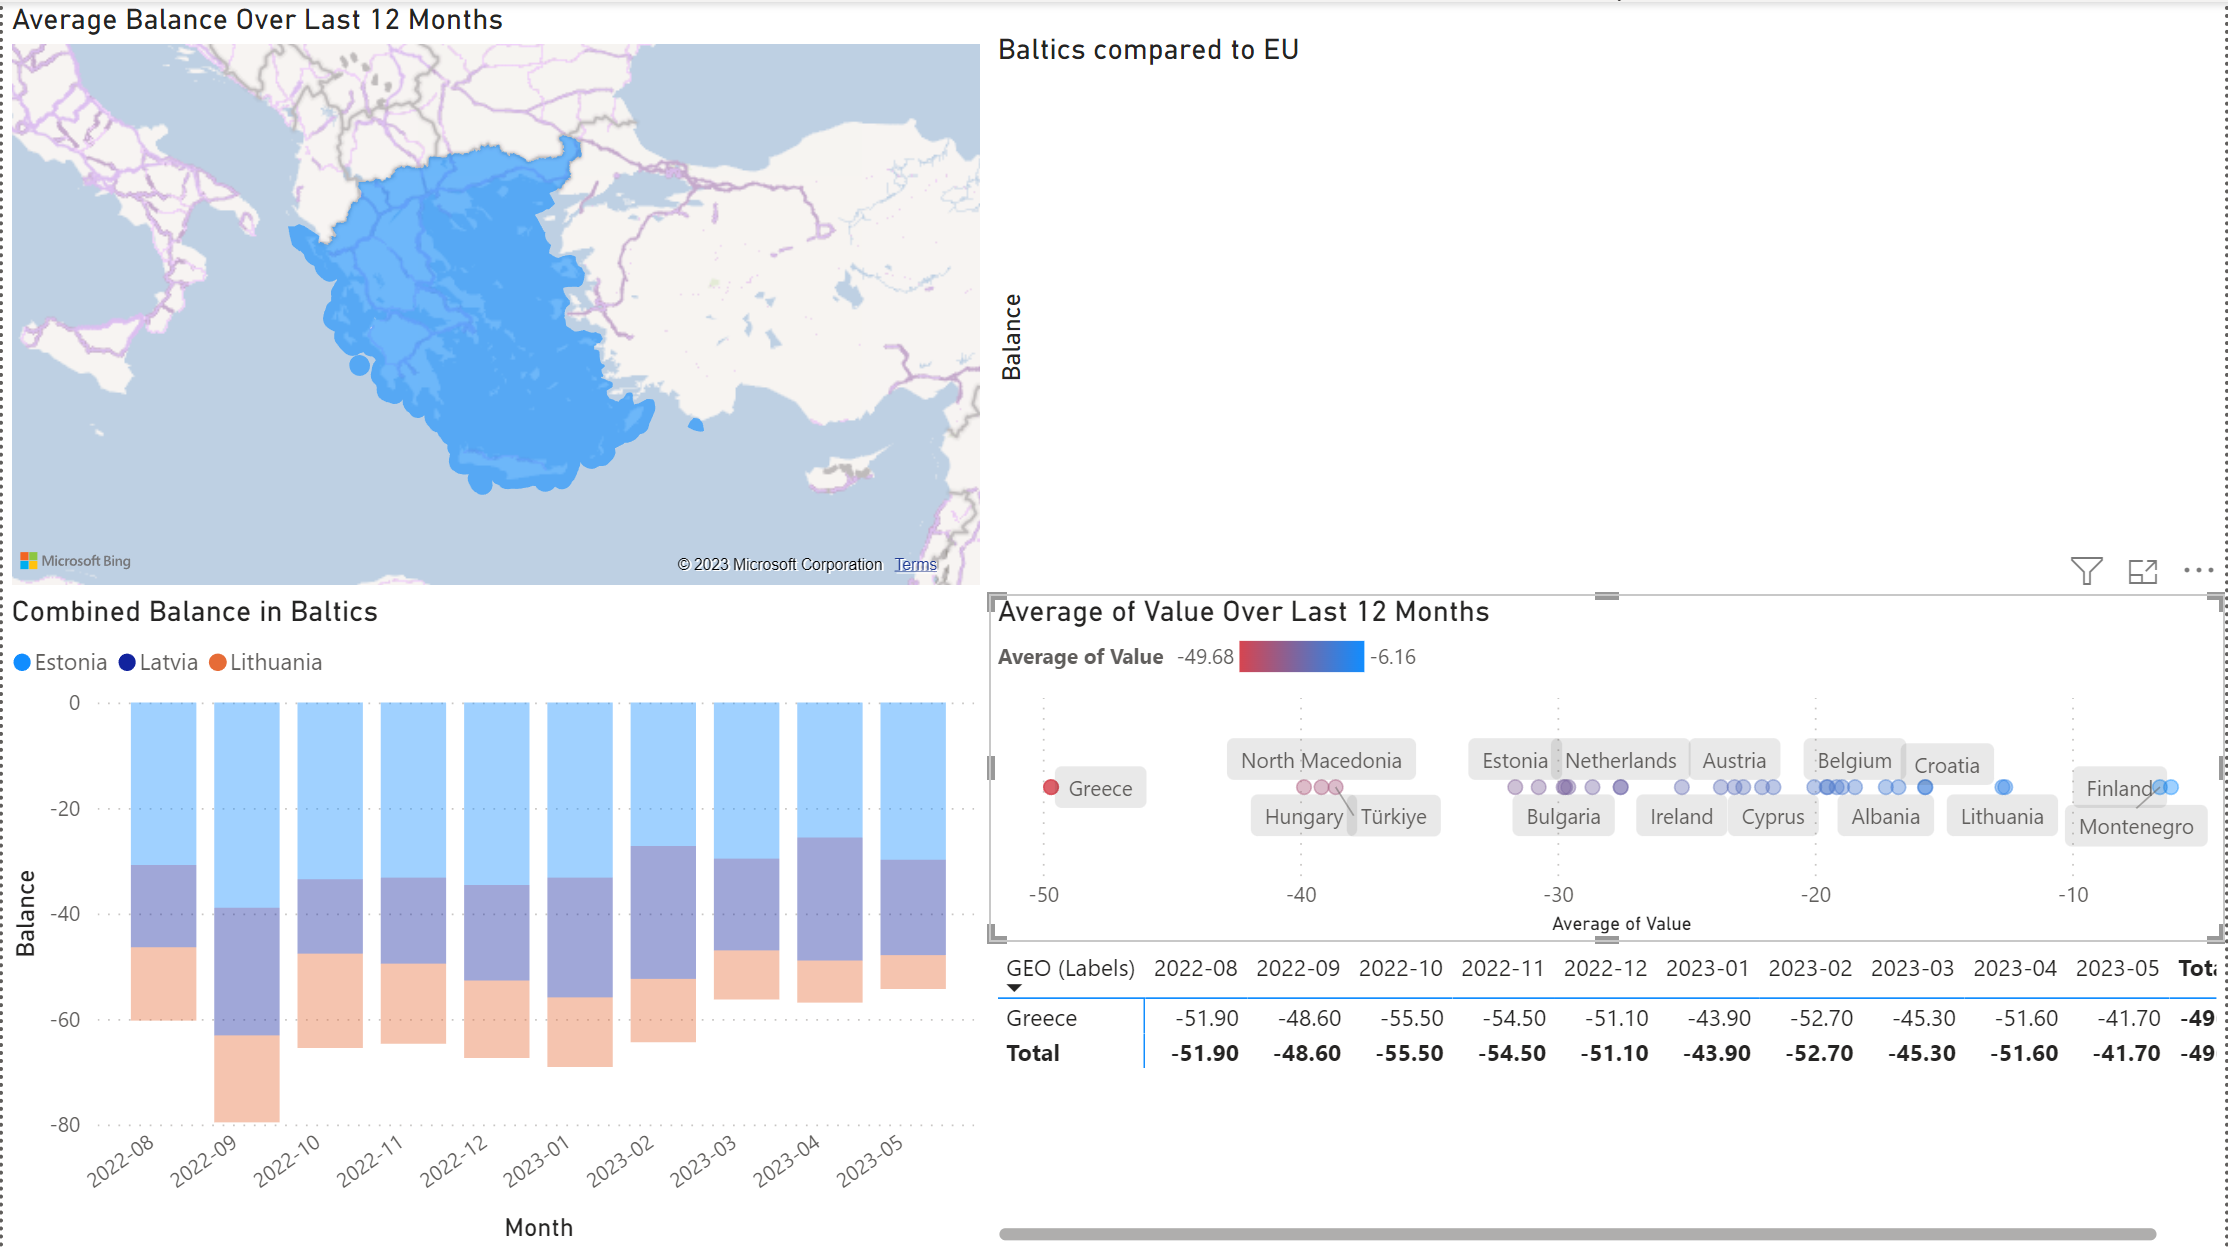
\includegraphics[width=0.9\textwidth, center]{Greece}

Projekts tika nopublicets.

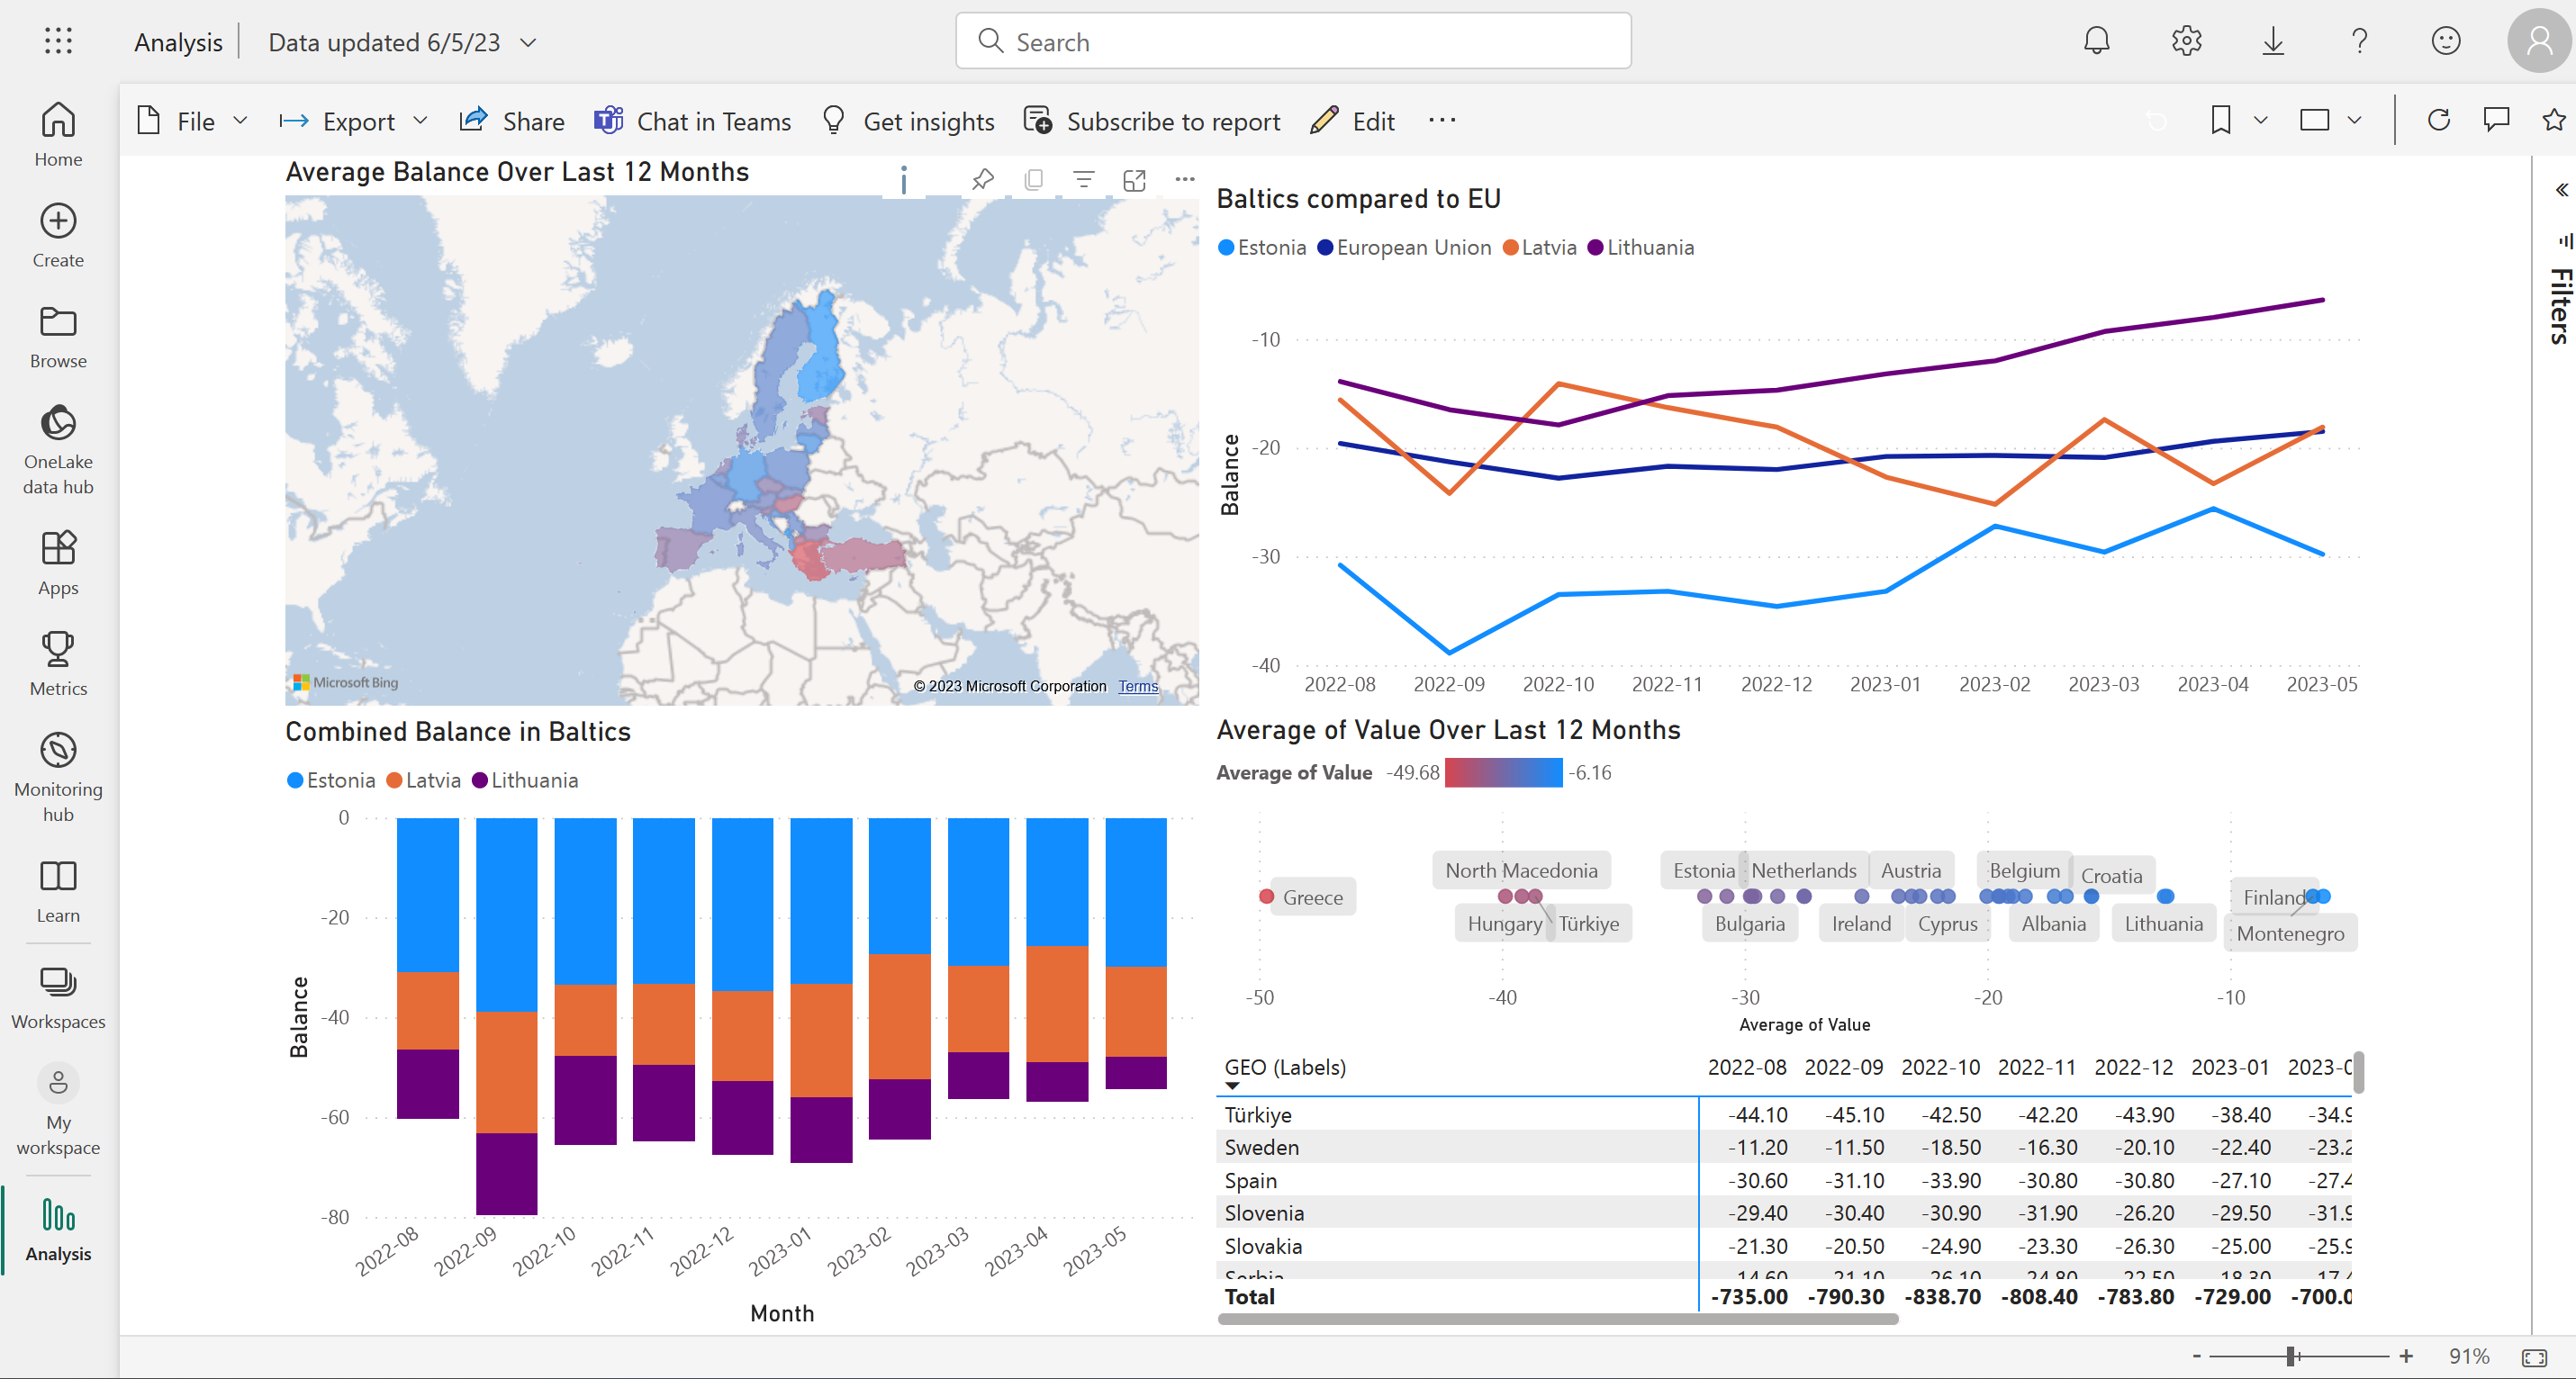
\includegraphics[width=0.9\textwidth, center]{Publish}

\section{Datu analīze/izvērtējums, secinājumi}
Kopumā var secināt, ka baltijas valstis ir labākā situācijā nekā pārējā eiropa. Un arī var redzēt, ka situācija ir uzlabojusies pēdējo 12 mēnešu laikā.

Papildus skatoties uz karti var redzēt, ka situācija ir labāka ziemeļos un sliktāka dienvidos.

\end{document}